\documentclass{book}
\usepackage{dsfont} %for \mathds command
%\usepackage{fullminipage}
\usepackage{epsfig}
\usepackage[cmex10]{amsmath}
\usepackage{graphicx}
\usepackage{pdfpages}
\usepackage{float}
\usepackage{amsfonts}
\usepackage{amsmath}
\usepackage{amssymb}
\usepackage{cite}
%\usepackage{floatrow}
\usepackage{bm}
\usepackage{mathrsfs}
\usepackage{subfig}
\usepackage{mathtools}
%\usepackage[ruled,vlined,linesnumbered]{algorithm2e}
\usepackage{arydshln}
\usepackage{inputenc}
\usepackage{algorithm}
\usepackage{algpseudocode}
%\usepackage{stfloats}
\usepackage{booktabs}
\newcommand*{\thead}[1]{\multicolumn{1}{c}{\bfseries #1}}
%\usepackage{algorithmic}
\usepackage{color}
\usepackage{amstext}
\usepackage{nomencl}
\usepackage{url}
\def\UrlBreaks{\do\/\do-}
\renewcommand{\UrlFont}{\small\tt}
\usepackage{multirow}
\usepackage{appendix}
\usepackage{verbatim}
\usepackage{longtable}
\usepackage{rotating}
\usepackage{fancyhdr}% fancyhdr related command; details in its documentation
%\graphicspath{{figures/}}
\DeclarePairedDelimiter{\abs}{\lvert}{\rvert}
\newcommand{\COMMENT}[1]{$\triangleright$  #1}


\begin{document}

\frontmatter

\title{ Adaptive Encoding for Constrained Video Delivery in HEVC, VP9, AV1 and VVC Compression Standards and
	Adaptation to Video Content}



\date{July 2020}

\maketitle

\mainmatter

%
%                       Chapter 1
%
\chapter{Introduction}
\label{ch1}

\begin{figure}[hbt!]
	\centering
	{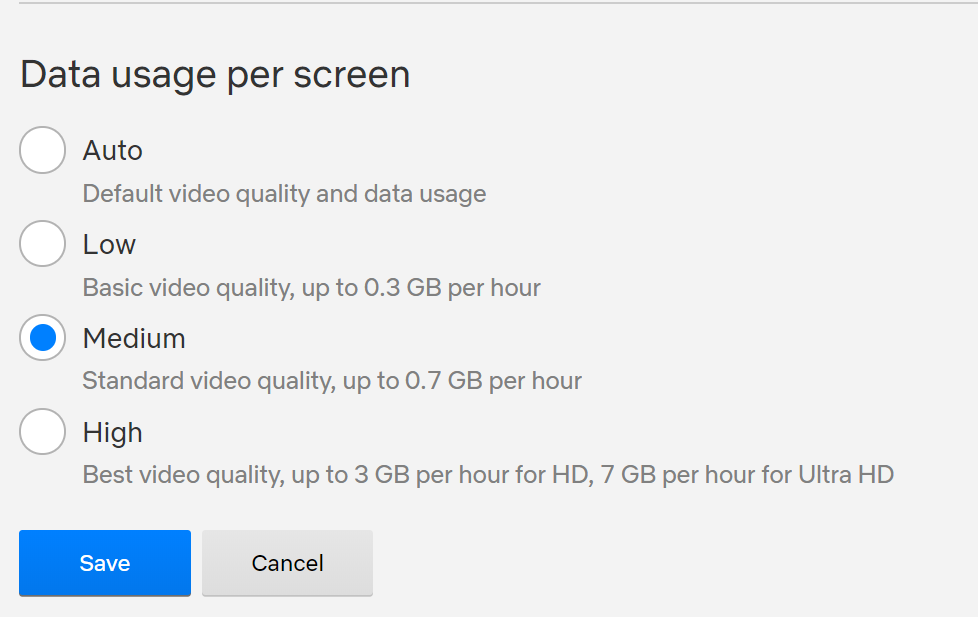
\includegraphics[width=0.80\textwidth]{pictures/ch1/Netflix_Video_Quality_settings.png}
		\label{fig:netflix_video}}
		\caption{Netflix Video Quality Settings}
\end{figure}
\newpage



%
%                                       Chapter 2
%
\chapter[Optimal GOP Configurations for x265 HEVC Encoder]{Optimal GOP Configurations for x265 HEVC Encoder in DRASTIC Framework}
   \begin{figure}[tb!]
   	\begin{minipage}{\columnwidth}
   		\begin{algorithmic}
   			\Function{\textbf{OptEnc}}{{\tt V}, {\tt Vc}, {\tt ParetoFront}, {\tt OptPars}} \\
   			\COMMENT {\textbf{Input:} video {\tt V}}, Pareto front in {\tt ParetoFront}, \\
   			\COMMENT {\hspace{0.25 true in}optimization mode specified in {\tt OptPars}.}  \\
   			\COMMENT {\textbf{Output:}  compressed video in {\tt Vc}.} \\
   			\State {\tt ParetoEntry} $\gets$ \textbf{Find} an optimal solution specified 
   			\State \hspace{0.6 true in} by {\tt OptPars} that lies on {\tt ParetoFront}.
   			\If{ (valid {\tt ParetoEntry} has been found)}
   			\State {\tt Vc} $\gets$ \textbf{Compress} {\tt V} using configuration
   			\State \hspace{0.25 true in} ({\tt P}, {\tt GOPconfig}, {\tt ParVec})
   			\State \hspace{0.25 true in} extracted from {\tt ParetoEntry}.
   			\Else 
   			\State {\tt ParetoEntry} $\gets$ \textbf{Search} {\tt ParetoFront} 
   			\State \hspace{0.25 true in} for an entry that violates the constraints by the
   			\State \hspace{0.25 true in} least amount. 
   			\State {\tt Vc} $\gets$ \textbf{Compress} {\tt V} using configuration
   			\State \hspace{0.25 true in} ({\tt P}, {\tt GOPconfig}, {\tt ParVec}) 
   			\State \hspace{0.25 true in} extracted from {\tt ParetoEntry}. 
   			\EndIf
   			\EndFunction
   		\end{algorithmic}
   	\end{minipage}
   	\caption{Optimal mode encoding using the Pareto front.
   	}\label{fig:Optimization}
   \end{figure}
  
\begin{figure}[hbt!]
	\centering
	 \subfloat[New GOP B4 configuration]
	 {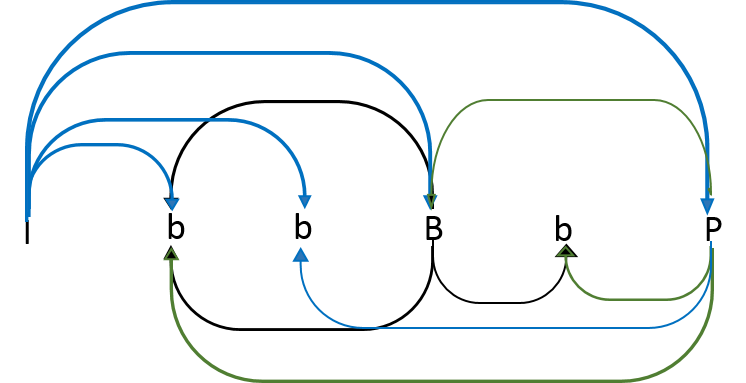
\includegraphics[width=0.5\textwidth]{pictures/ch2/x265_B4_GOP1.png}
		\label{fig:x265_B4_GOP1}}
	\subfloat[New GOP B2 configuration]
	{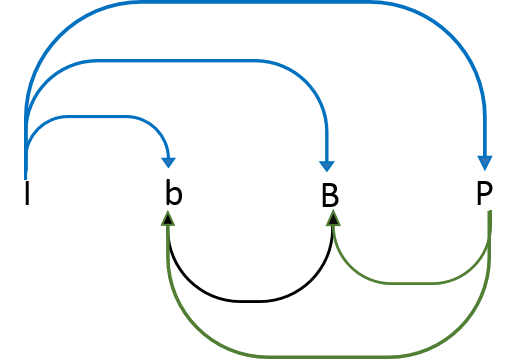
\includegraphics[width=0.4\textwidth]{pictures/ch2/x265_B2_GOP.png}
		\label{fig:x265_B2_GOP}} \\
	
	\subfloat[New GOP B6 configuration]
	{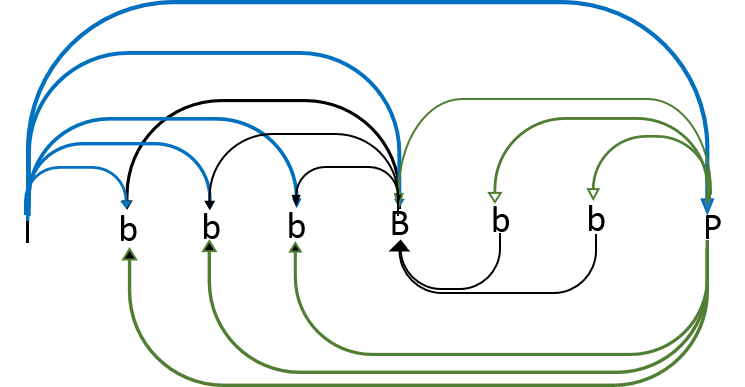
\includegraphics[width=0.6\textwidth]{pictures/ch2/x265_B6_GOP.png}
		\label{fig:x265_B6_GOP}}
	\caption{New GOP configurations. % (a) Default GOP configuration (B4).
		(a) Extended GOP configuration by removing a \textbf{b} frame.
		(b) Extended GOP configuration by adding a \textbf{b} frame.}     
	\label{fig:newGOPs}
\end{figure}

\begin{figure}[bh!]
	\centering
	\subfloat[Jockey \cite{UHDvideo}.]
	{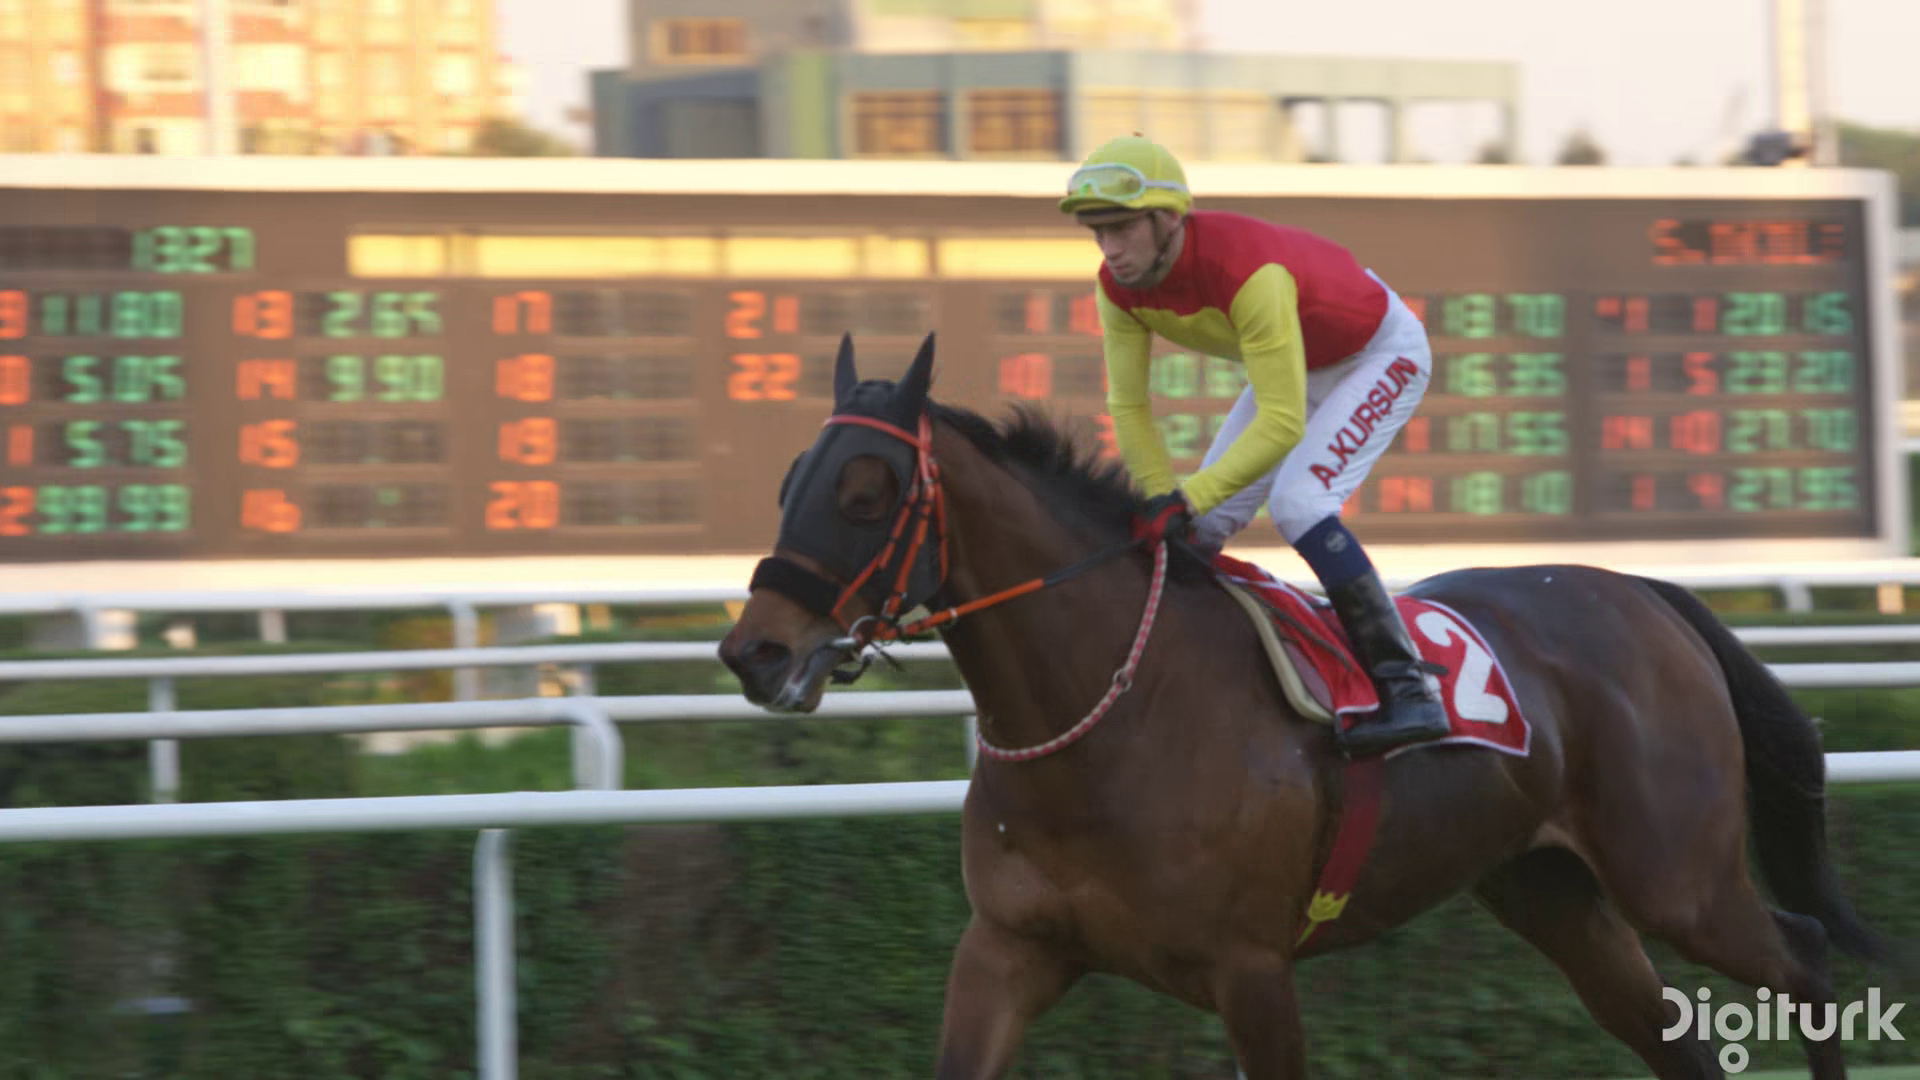
\includegraphics[width=1.9 true in]{pictures/ch2/2KJockey1920x1080.png}
		\label{fig:nonBovik}} 
	\subfloat[Pedestrian \cite{Kalpana,Seshadrinathan}.]
	{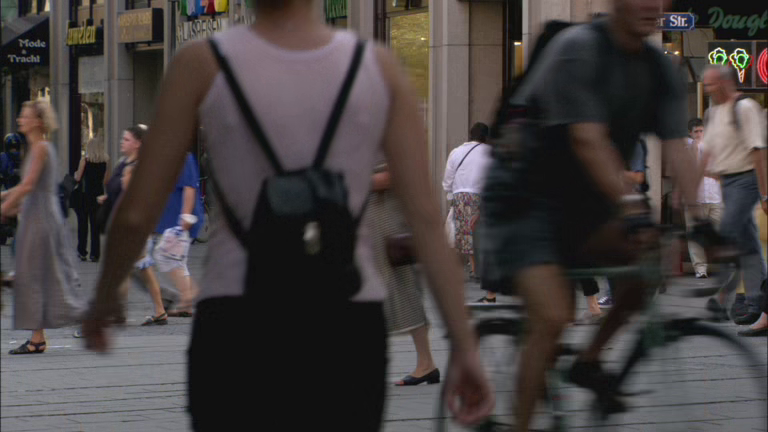
\includegraphics[width=1.9 true in]{pictures/ch2/Pedestrian768x432.png}
		\label{fig:Bovik1}} 			
	\subfloat[Riverbed \cite{Kalpana,Seshadrinathan}.] 
	{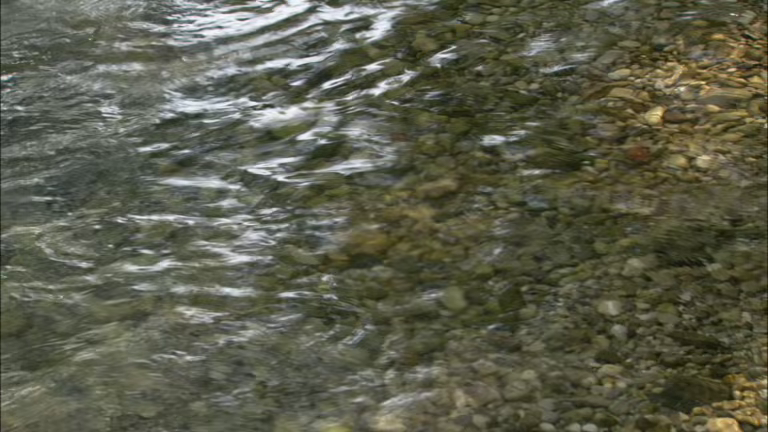
\includegraphics[width=1.9 true in]{pictures/ch2/Riverbed.png}
		\label{fig:Bovik2}} 
	\\		
	%trim option's parameter order: left bottom right top
	\subfloat[Pareto front for UHD video: Jockey (1920x1080, 30 fps, 150 frames).]		
	{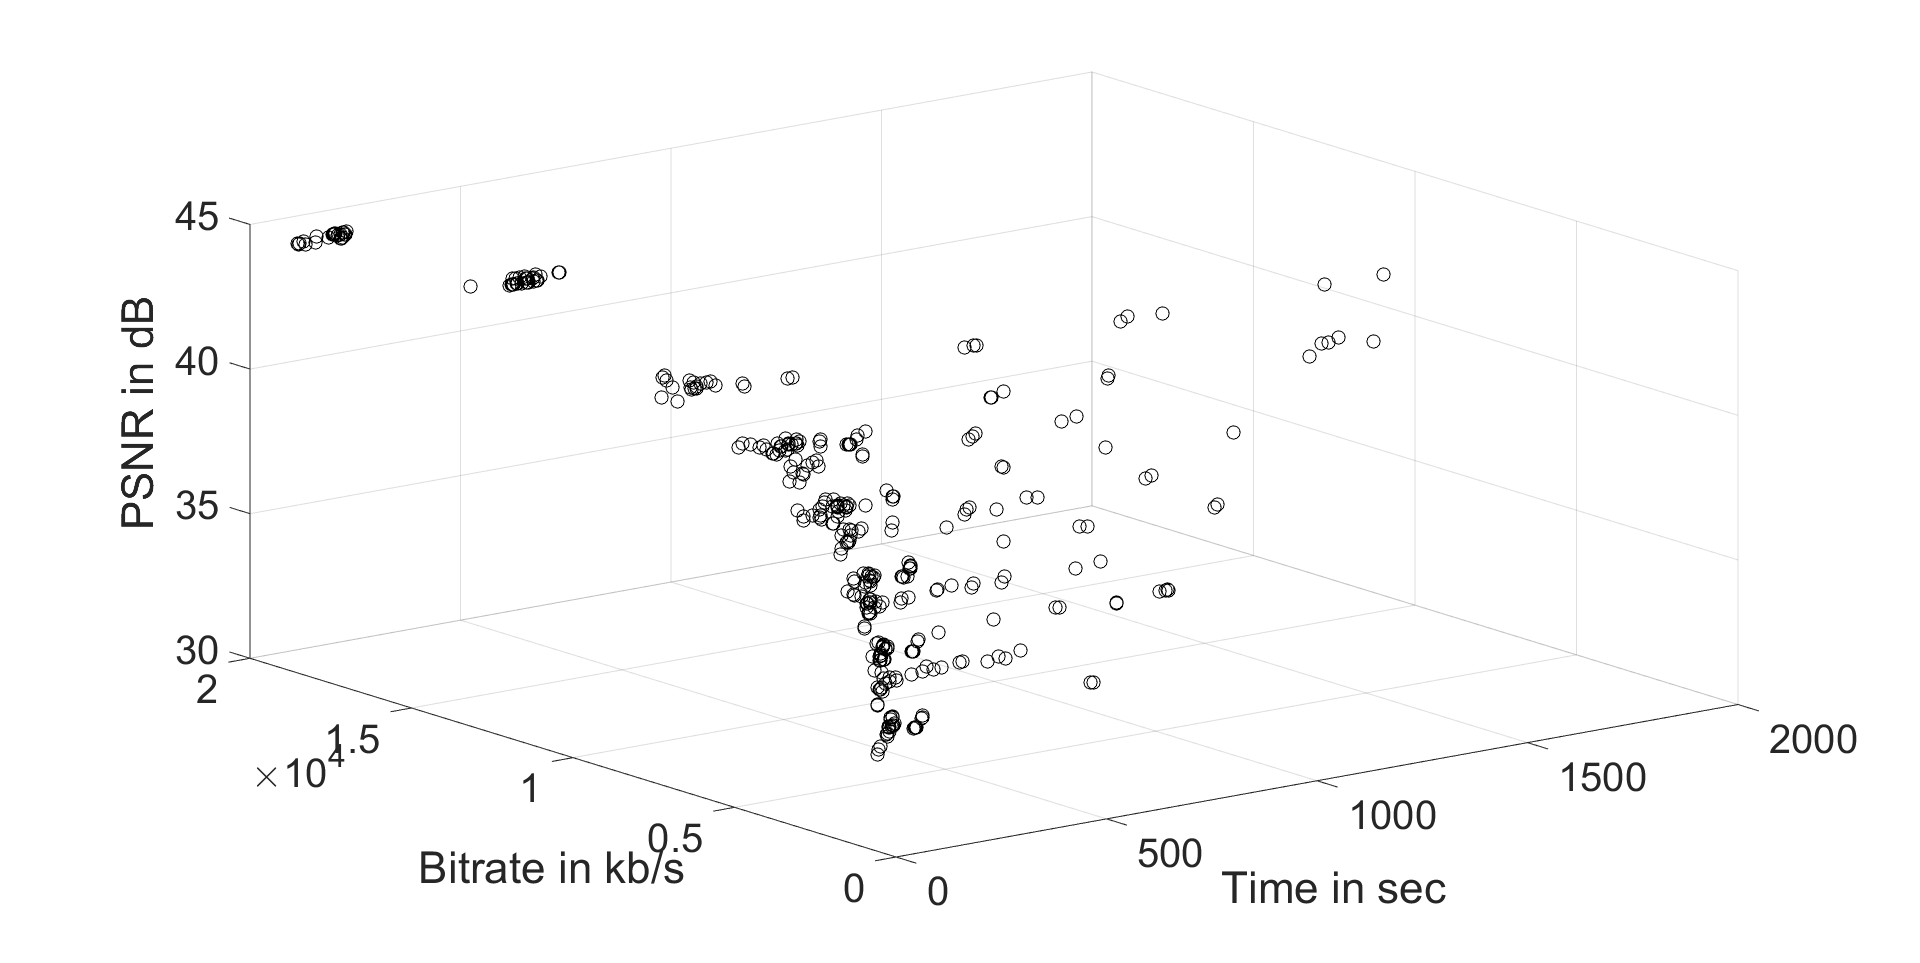
\includegraphics[trim=20mm 10mm 25mm 25mm, clip, width=0.4\textwidth]{pictures/ch2/Pareto_Jockey.png}
		\label{fig:P1}} \\
	\subfloat[Pareto Front for Pedestrian video (768x432, 25 fps, 250 frames).]
	{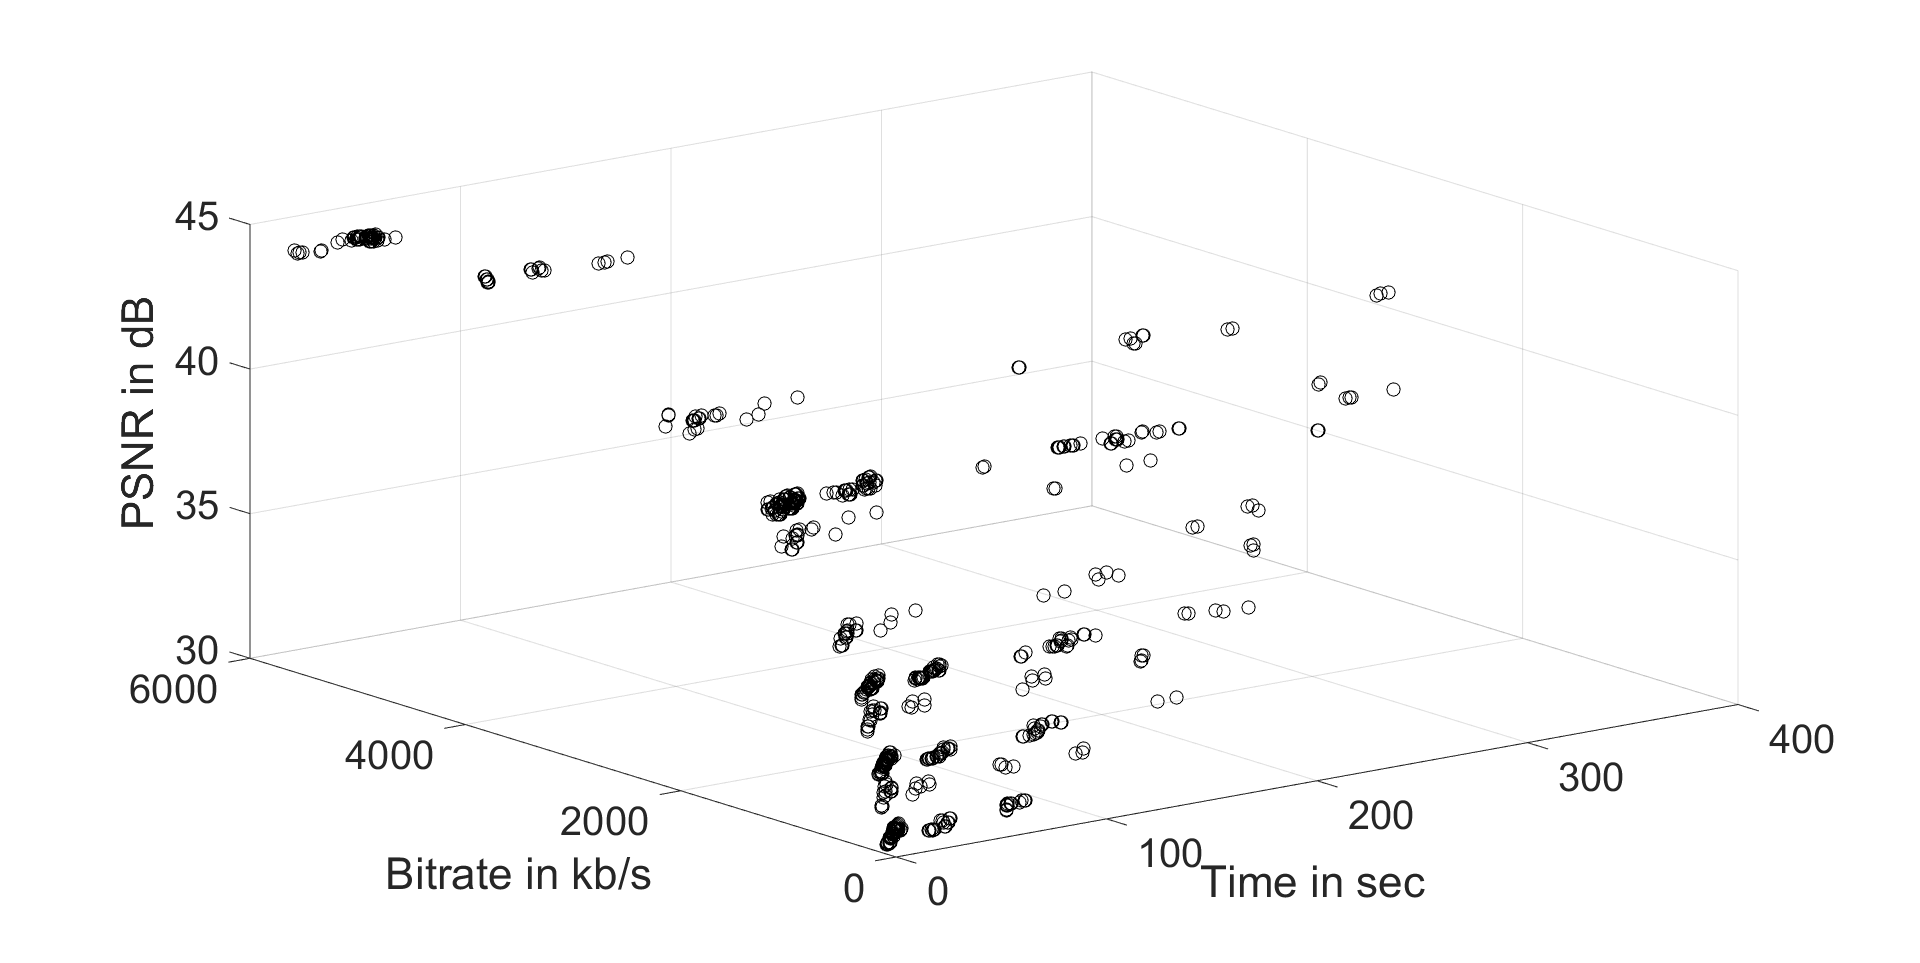
\includegraphics[trim=20mm 10mm 25mm 25mm, clip, width=0.4\textwidth]{pictures/ch2/Pareto_Pa.png}
		\label{fig:P2}} \\
	\subfloat[Pareto Front for Riverbed video 768x432]
	{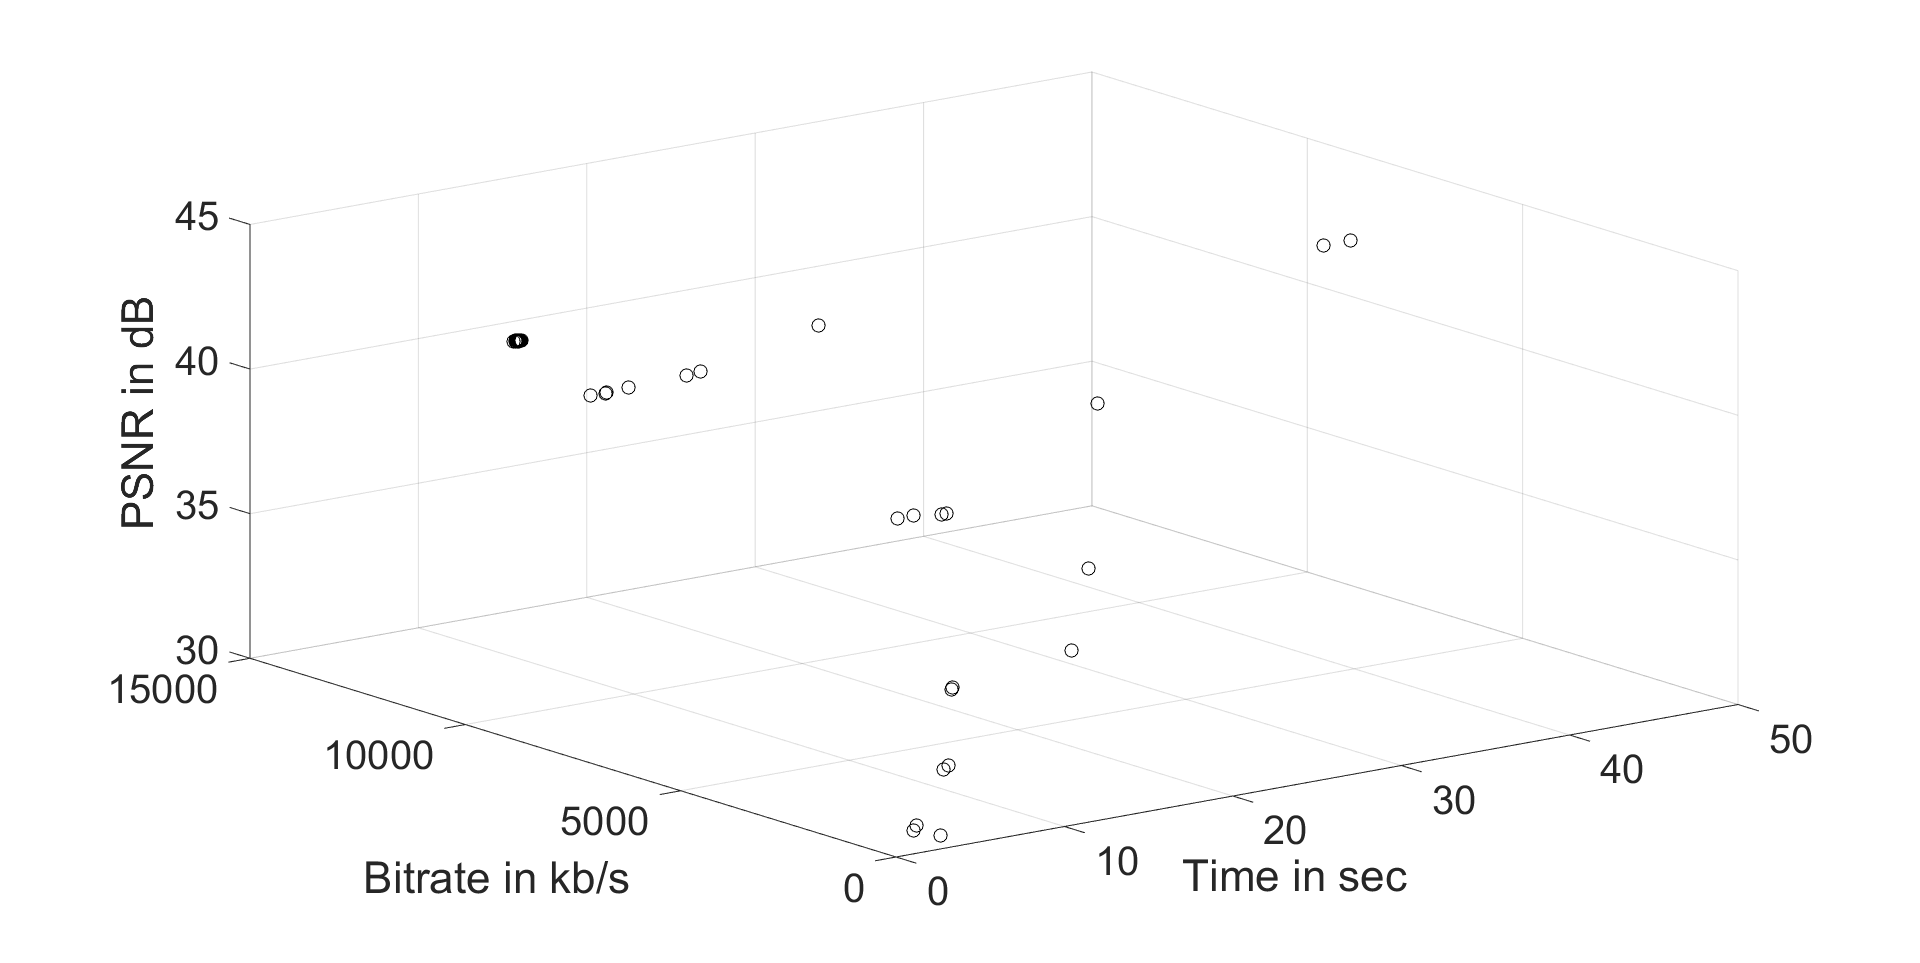
\includegraphics[width=0.5\textwidth]{pictures/ch2/Pareto_Rb.png}
		\label{fig:subfigure1}} \\		
	
	\caption{ Test videos and resulting Pareto fronts. 
		(a) UHD video with strong predictable, translational motions. 
		(b) Pedestrian video with multiple, yet predictable, translational motions.
		(c) Riverbed video with very complicated motions created by the flowing water.
		(d) Pareto front for UHD video demonstrating a relatively dense front.
		(e) Pareto front for Pedestrian video demonstrating a relatively dense front.  (f) Pareto front for Riverbed video with fewer optimal points on pareto front.}
	\label{fig1:setup}                 
\end{figure}






%
%                       Chapter 3
%
\chapter{ Adaptive video encoding based on Camera activity Classification}
\label{chap:3}
\begin{figure}[t!]
	\centering
	\subfloat[]
	{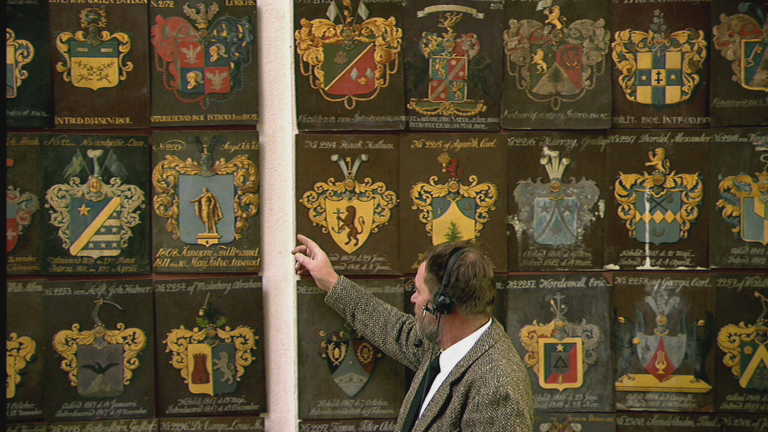
\includegraphics[width=1.6 true in]{pictures/ch3/ShieldTrack.png}
		\label{fig:ShieldTrack}}
	\subfloat[]
	{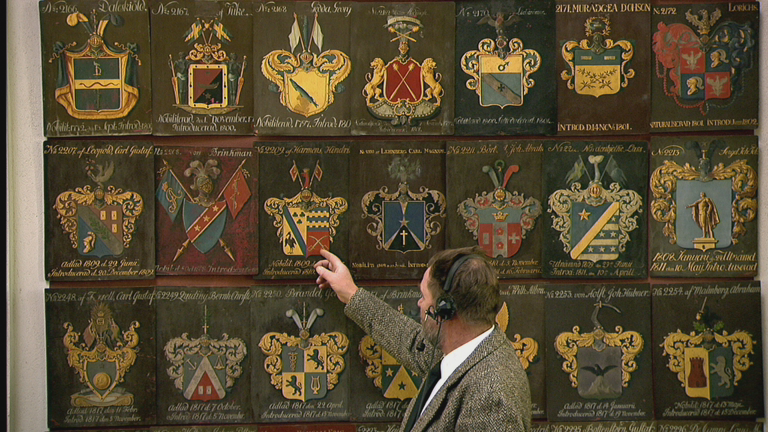
\includegraphics[width=1.6 true in]{pictures/ch3/ShieldStationary.png}
		\label{fig:ShieldStationary}} 			
	\subfloat[]
	{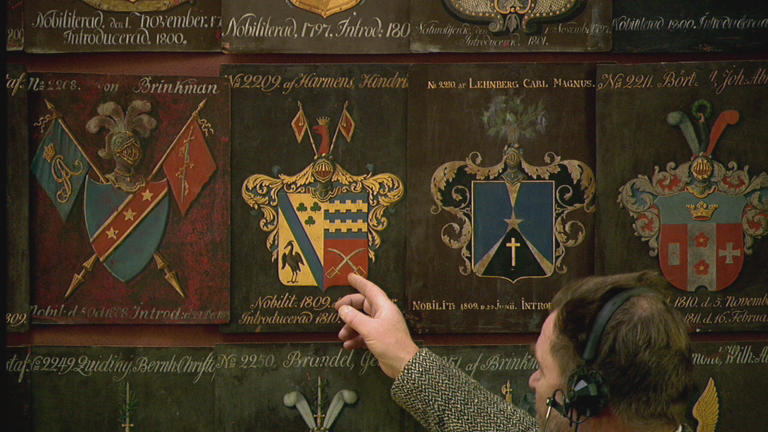
\includegraphics[width=1.6 true in]{pictures/ch3/ShieldZoom.png}
		\label{fig:shield}} \\
	\caption{\label{fig:shields}
		Test video Shields from UT LIVE Video Quality Database \cite{Kalpana}.
		(a) Camera moving as the man is pointing his finger at different shield images.
		(b) Camera remains stationary over the target shield image.
		(c) Camera zooming in the particular shield that is of interest.}
\end{figure}

\begin{figure}[b!]
	\centering
	\subfloat[]
	{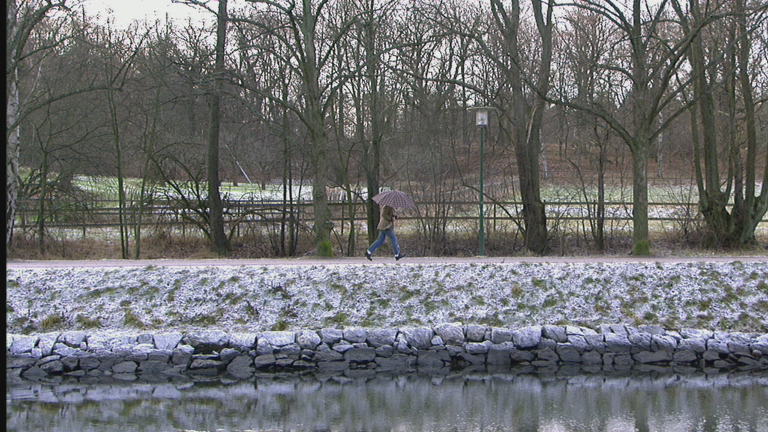
\includegraphics[width=1.7 true in]{pictures/ch3/ParkRunTrack.png}
		\label{fig:ParkRunTrack}}
	\subfloat[]
	{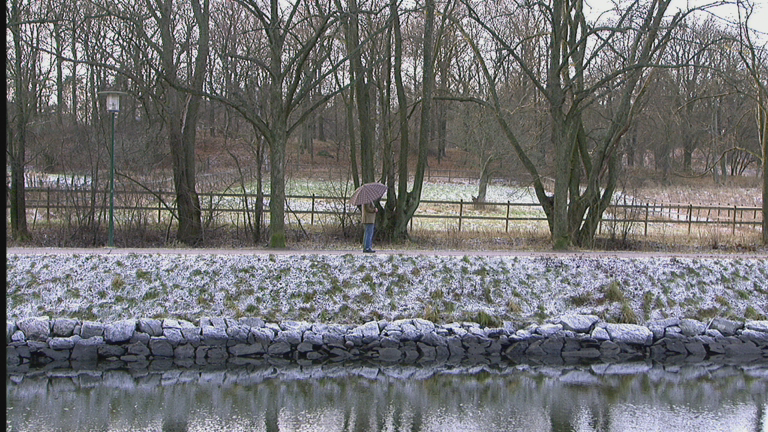
\includegraphics[width=1.7 true in]{pictures/ch3/ParkRunStationary.png}
		\label{fig:parkrun1}} \\
	\caption{\label{fig:parkrun}
		Test video Parkrun from UT LIVE Video Quality Database \cite{Kalpana}.
		(a) Camera moving and tracking the man during a running activity.
		(b) Camera remains stationary when the man stops running.}
\end{figure}

\begin{figure}[hbt!]
	\centering
	{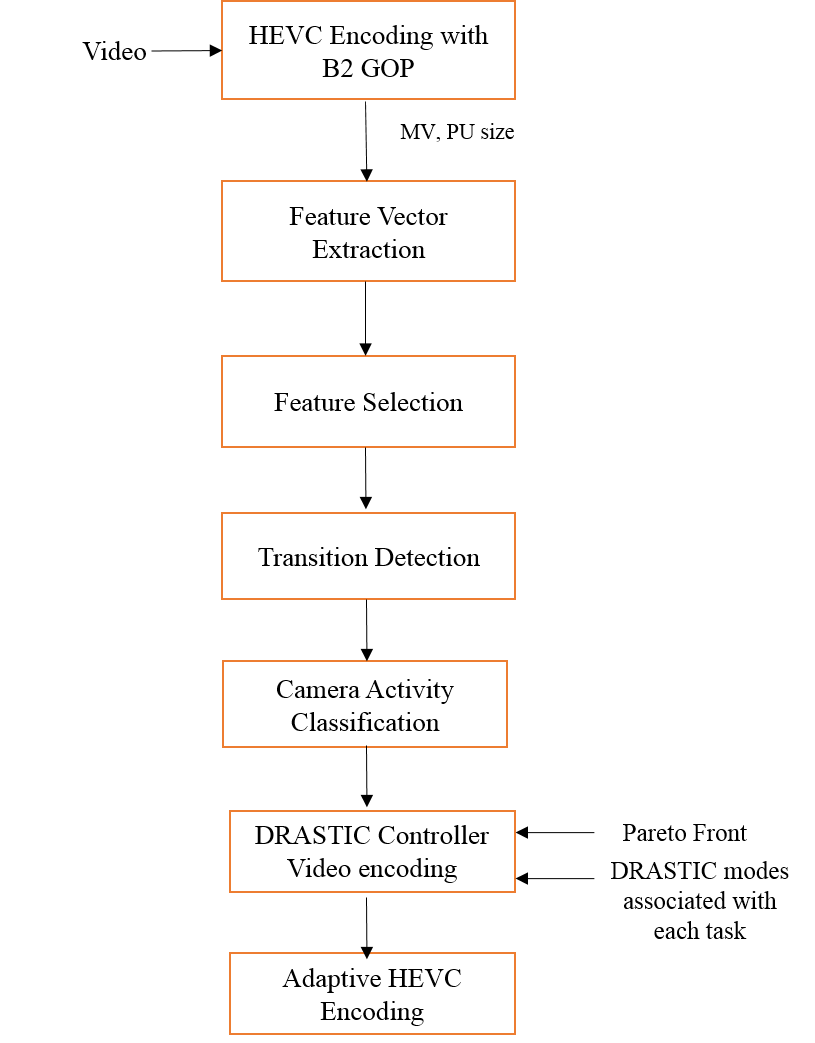
\includegraphics[width=0.95\linewidth]{pictures/ch3/pic1.png}
		\label{fig:blkdia1}}
	\caption{Block Diagram of Video activity detection with Classifier.}
\end{figure}

\begin{figure*}
	% trim={<left> <lower> <right> <upper>}
	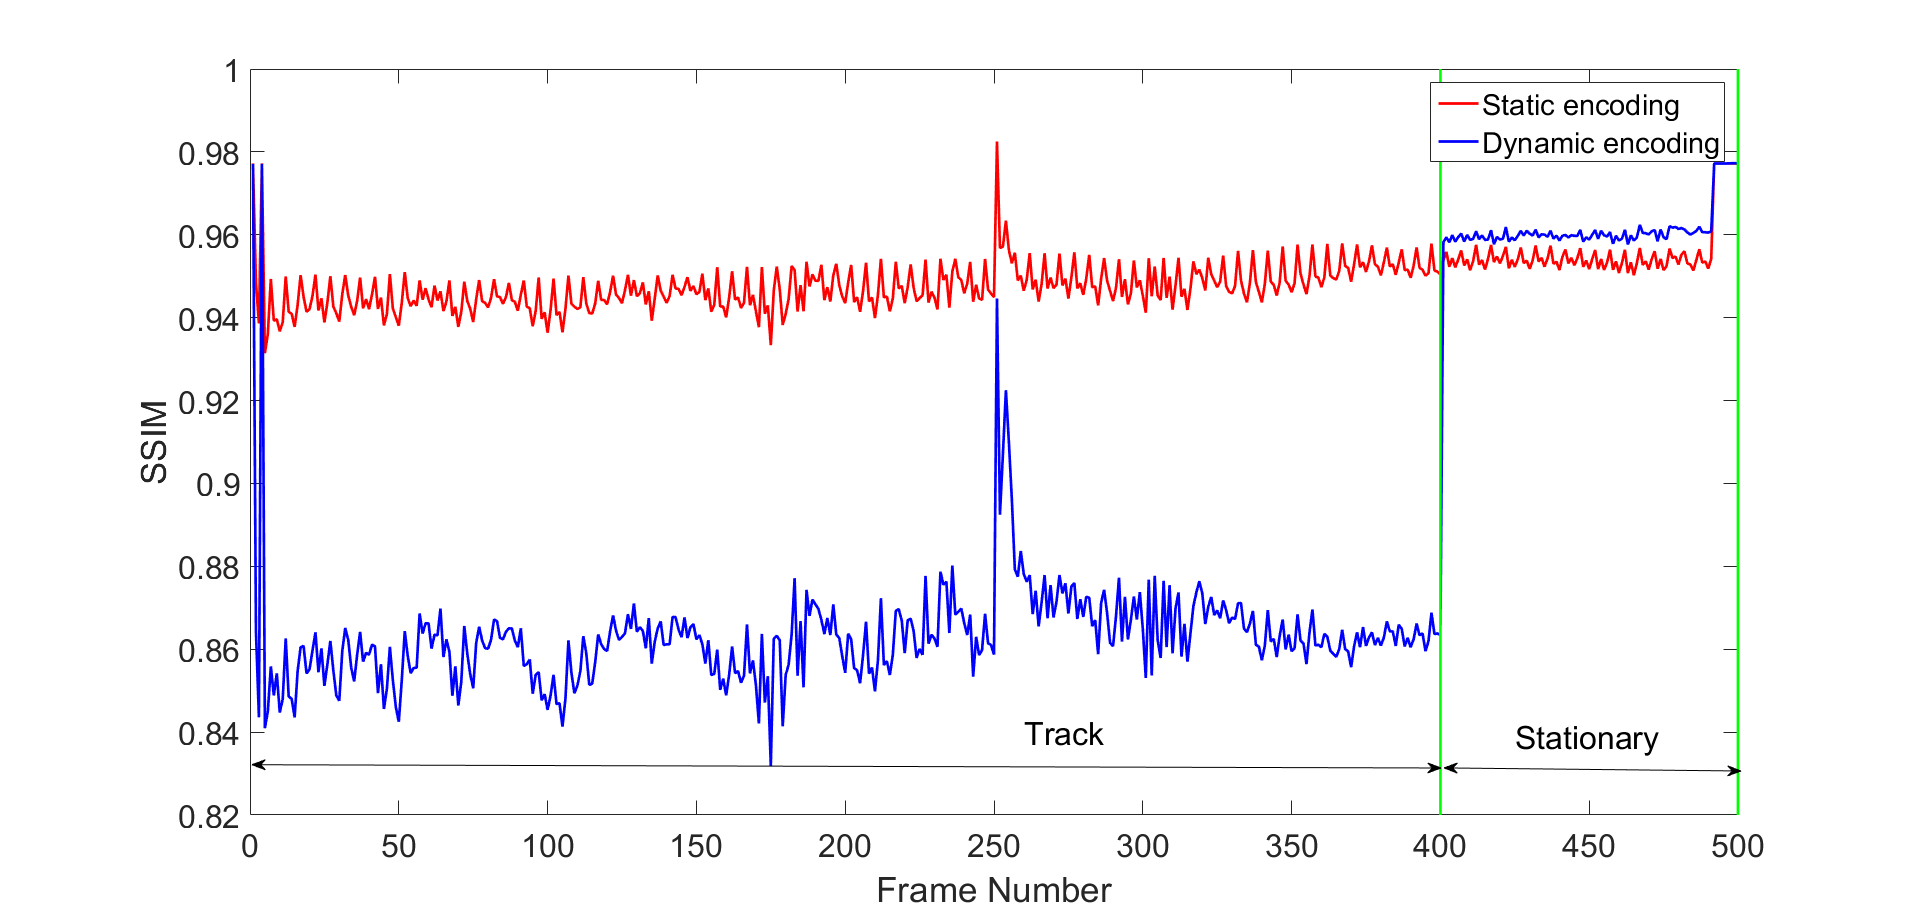
\includegraphics[width=\linewidth, clip]{pictures/ch3/Pr_TrackingLessImportant.png}
	\caption{\label{fig:adaptiveEncPr}
		Adaptive video encoding example for the Parkrun video from the 
		UT LIVE Video Quality Database \cite{Kalpana}.
		Refer to table \ref{tbl:adaptive} for the bitrate constraints.
		Bitrate savings results from reducing the SSIM video quality
		constraint over the stationary portion of the video.
	}
\end{figure*}

\begin{figure*}
	% trim={<left> <lower> <right> <upper>}
	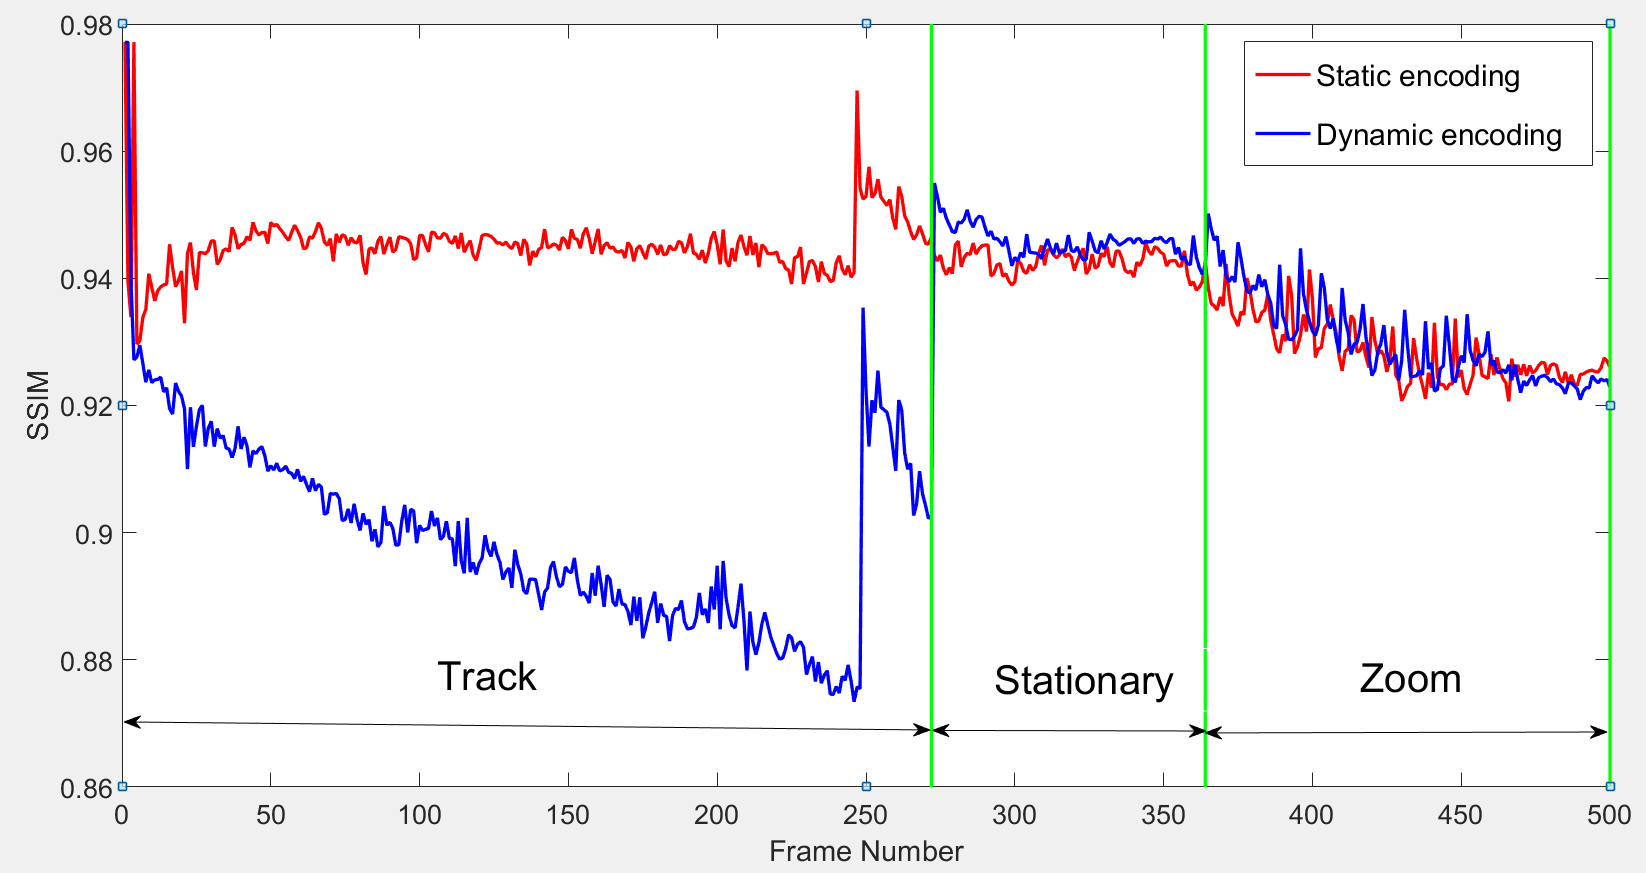
\includegraphics[width=\linewidth, clip]{pictures/ch3/ShieldSSIM.png}
	\caption{\label{fig:adaptiveEncSh}
		Adaptive video encoding example for the Parkrun video from the 
		UT LIVE Video Quality Database \cite{Kalpana}.
		Refer to table \ref{tbl:adaptive} for the bitrate constraints.
		Bitrate savings results from reducing the SSIM video quality
		constraint over the stationary portion of the video.
	}
\end{figure*}





%
%                       Chapter 4
%
\chapter[Segment based x265 encoding with adaptive Local Pareto models for VoD]{Segment based x265 encoding with adaptive Local Pareto models for  Video On Demand (VoD)}


\begin{figure}[hbt!]
    
     	{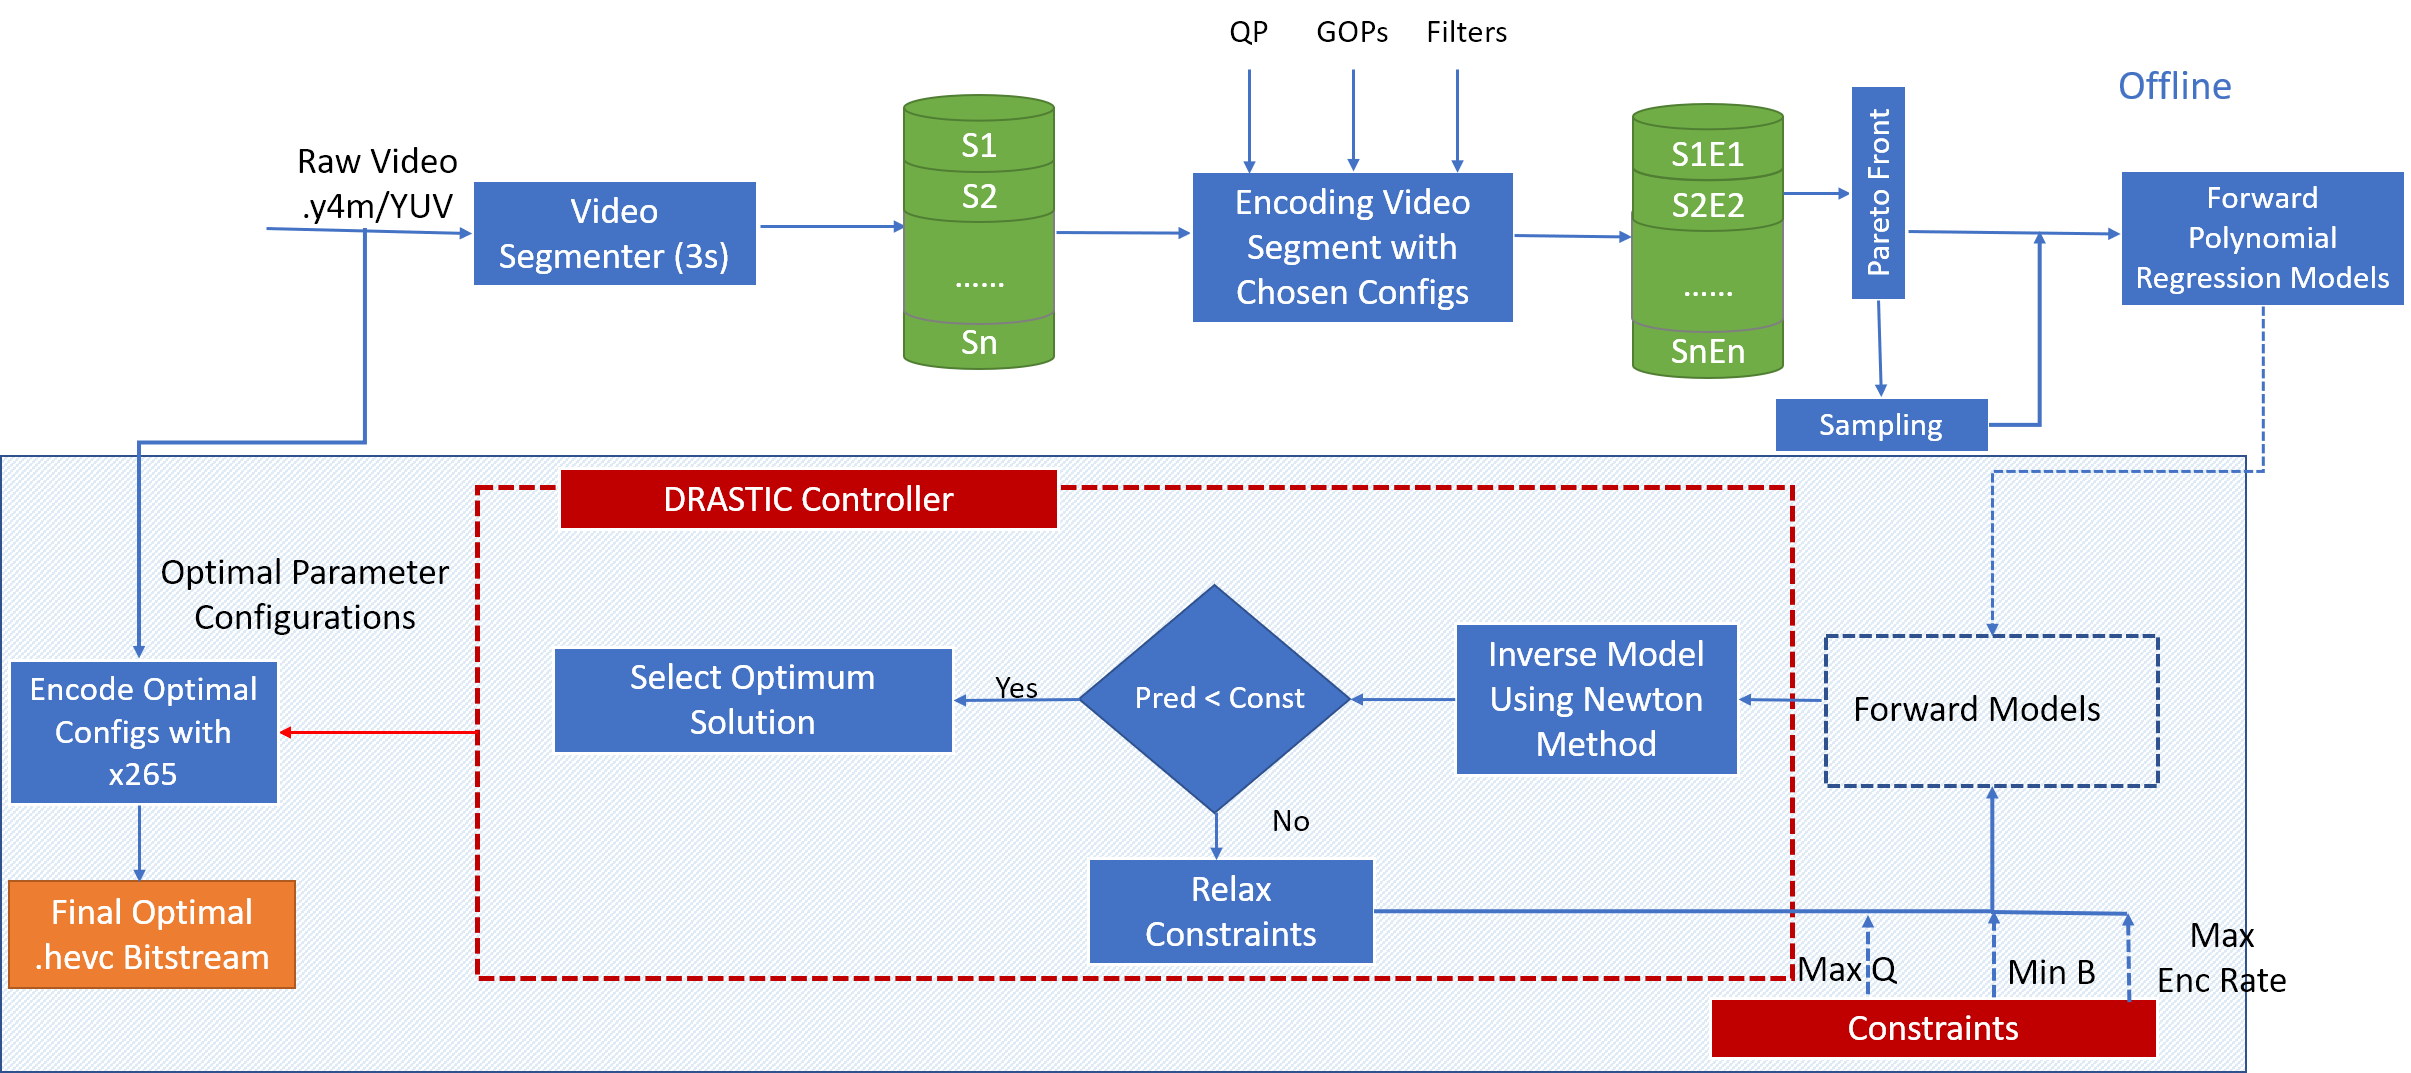
\includegraphics[width=\columnwidth]{pictures/ch4/DRASTIC_x265_Seg_Enc.png}\\
     		\label{fig:Segblkdiag}}
     	\caption{Block Diagram of Segment based Local Pareto models with DRASTIC Control modes.}
\end{figure}
     
 
    
\begin{figure}[bt!]
	\centering
	\subfloat[]
	{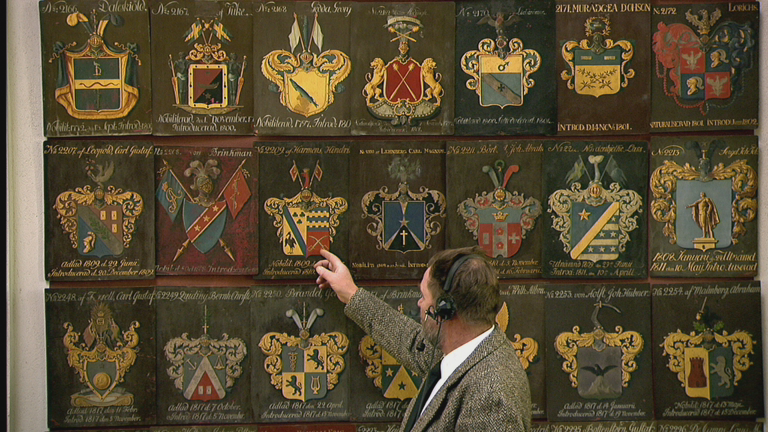
\includegraphics[width=1.9 true in]{pictures/ch4/Shields_UTLIVE.png}
		\label{fig:Ch4Shields_UTLIVE}}
	\subfloat[]
	{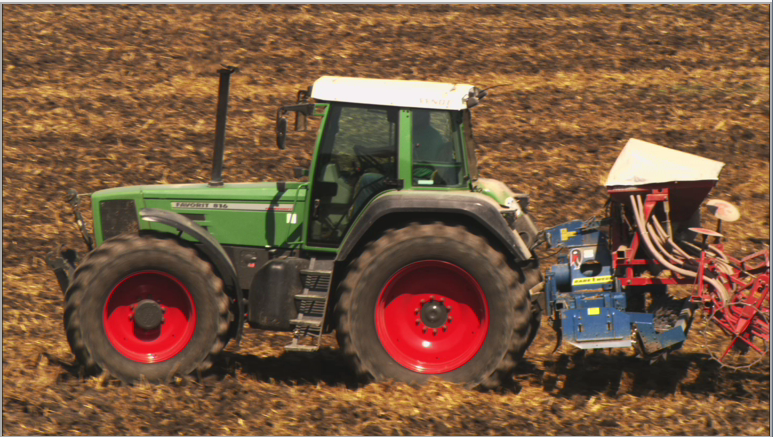
\includegraphics[width=1.9 true in]{pictures/ch4/Tractor_UTLIVE.png}
		\label{fig:Ch4Tractor_UTLIVE}} 			
	\subfloat[]
	{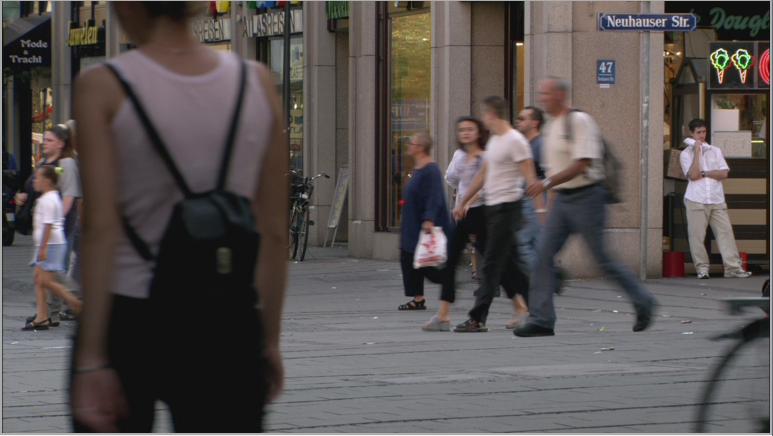
\includegraphics[width=1.9 true in]{pictures/ch4/Pedes_UTLIVE.png}
		\label{fig:Ch4Pedes_UTLIVE}} \\
	\subfloat[]
	{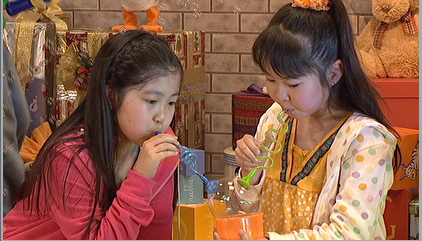
\includegraphics[width=1.9 true in]{pictures/ch4/HEVC_ClassD240.png}
		\label{fig:Ch4Bubbles}} 
	\subfloat[]
	{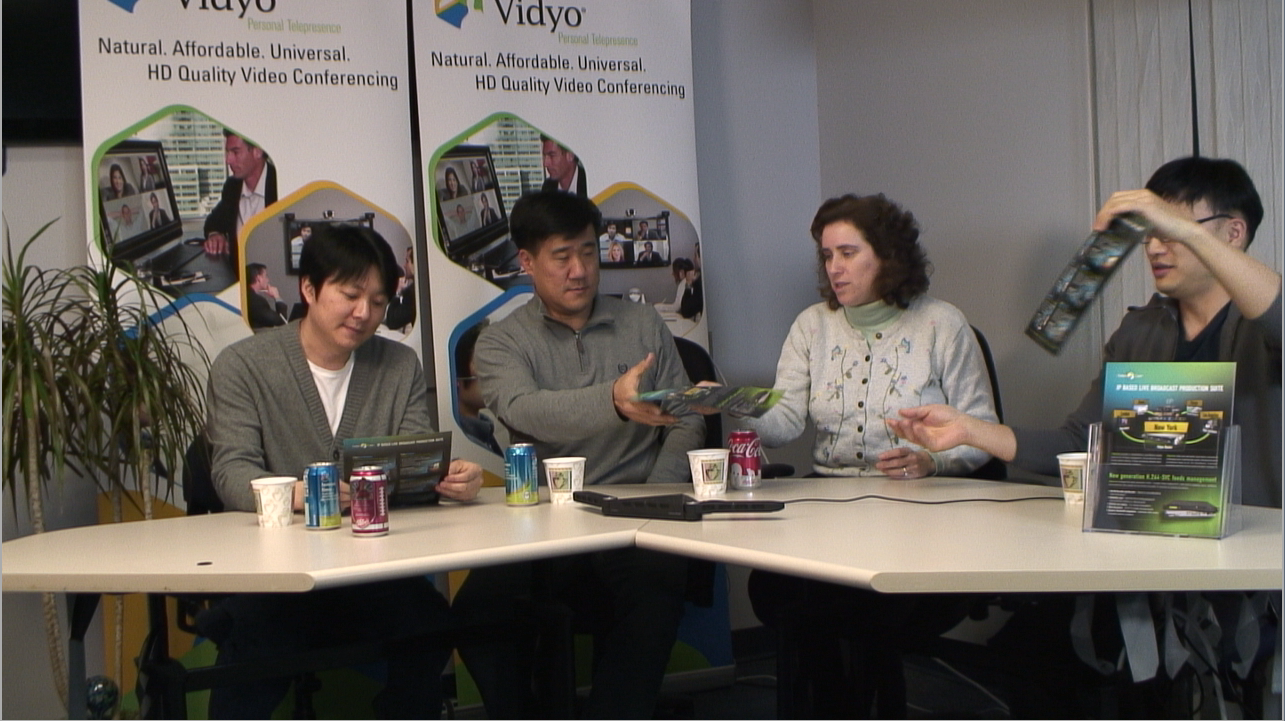
\includegraphics[width=1.9 true in]{pictures/ch4/HEVC_ClassE.png}
		\label{fig:Ch4Fourppl}} 
	\subfloat[]
	{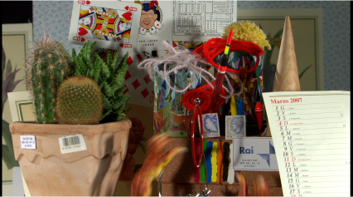
\includegraphics[width=1.9 true in]{pictures/ch4/HEVC_ClassB.png}
		\label{fig:Ch4Cac}} \\
	\subfloat[]
	{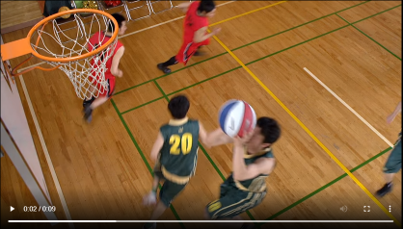
\includegraphics[width=1.9 true in]{pictures/ch4/HEVC_ClassC.png}
		\label{fig:Ch4BBDrill}}	
    \subfloat[]
    {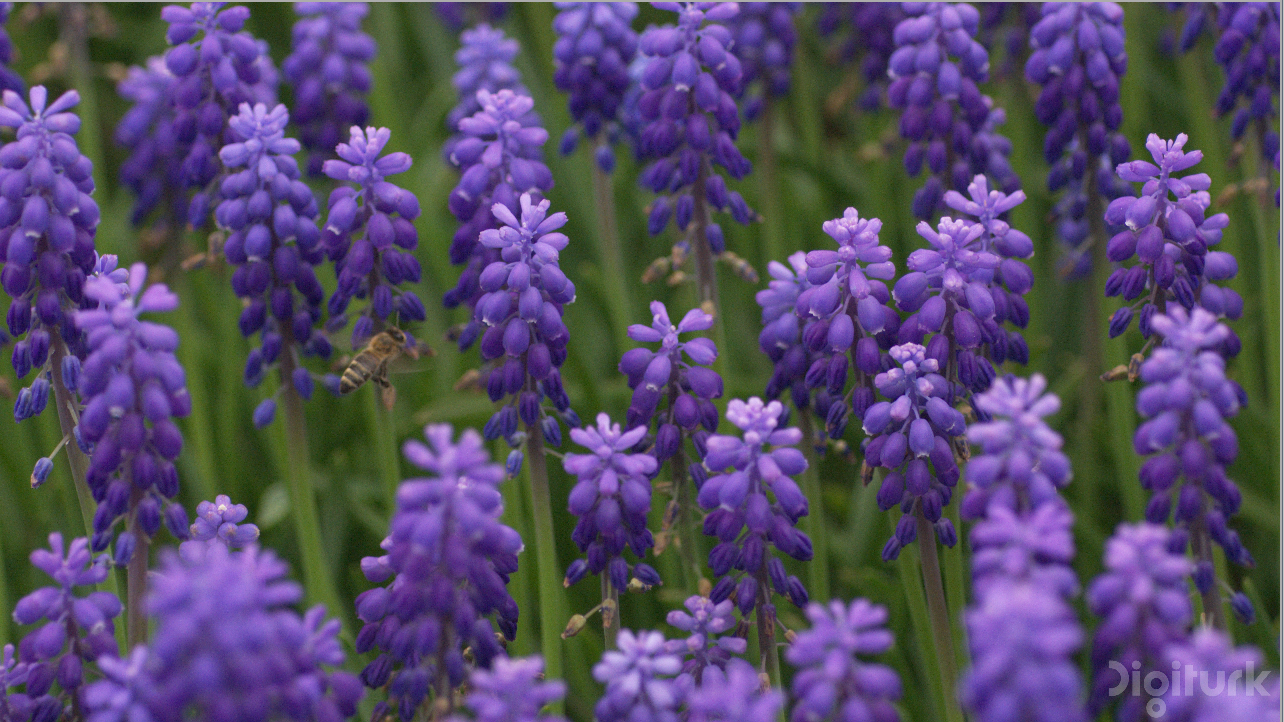
\includegraphics[width=1.9 true in]{pictures/ch4/HoneyBeeUHD.png}
    	\label{fig:Ch4HB}}
    \subfloat[]
	{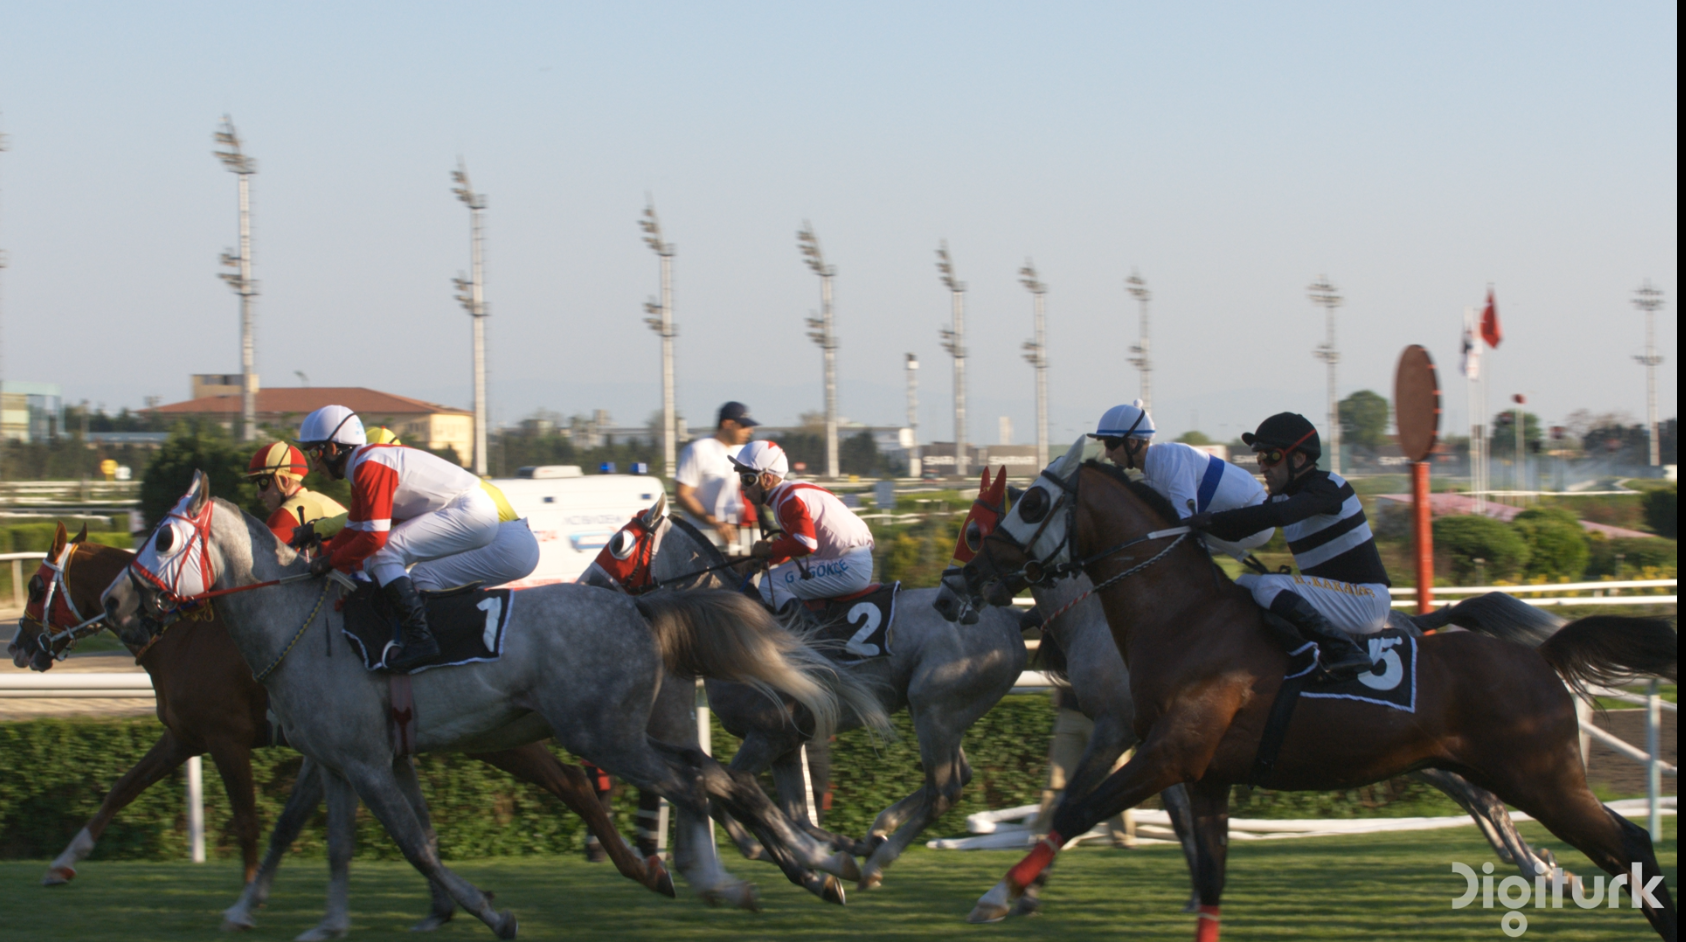
\includegraphics[width=1.9 true in]{pictures/ch4/ReadysetGoUHD.png}
		\label{fig:Ch4RSG}}

	 
	\caption{\label{fig:x265Video_Databases}
		Test video Shields from UT LIVE Video Quality Database \cite{Kalpana}
		 %UT LIVE % FOr other Databases insert references %
		(a),(b),(c) Shields, Tractor, Pedestrian video with resolution 768x432 of 50, 25,25 fps respectively  from UT LIVE Video Quality Database .
		(d) Blowing Bubbles of 480x240 from Class D with 50fps,
		(e) Four People with resolution 1280x720 from Class E with 60fps from HEVC Standard Test video sequences.
		(f), (g) Cactus, BasketballDrill video with resolution 1920x1080,50 fps and 832x480, 50fps respectively from HEVC \cite{HEVCTestvideo} Video Test sequences.
		(h), (i) HoneyBee, ReadysetGo videos with resolution 1920x1080, 60 fps publicly available from Ultra Video group, Tampere \cite{UHDvideo} University.
		}	
\end{figure}

\begin{figure}[hbt!]
	\centering
	{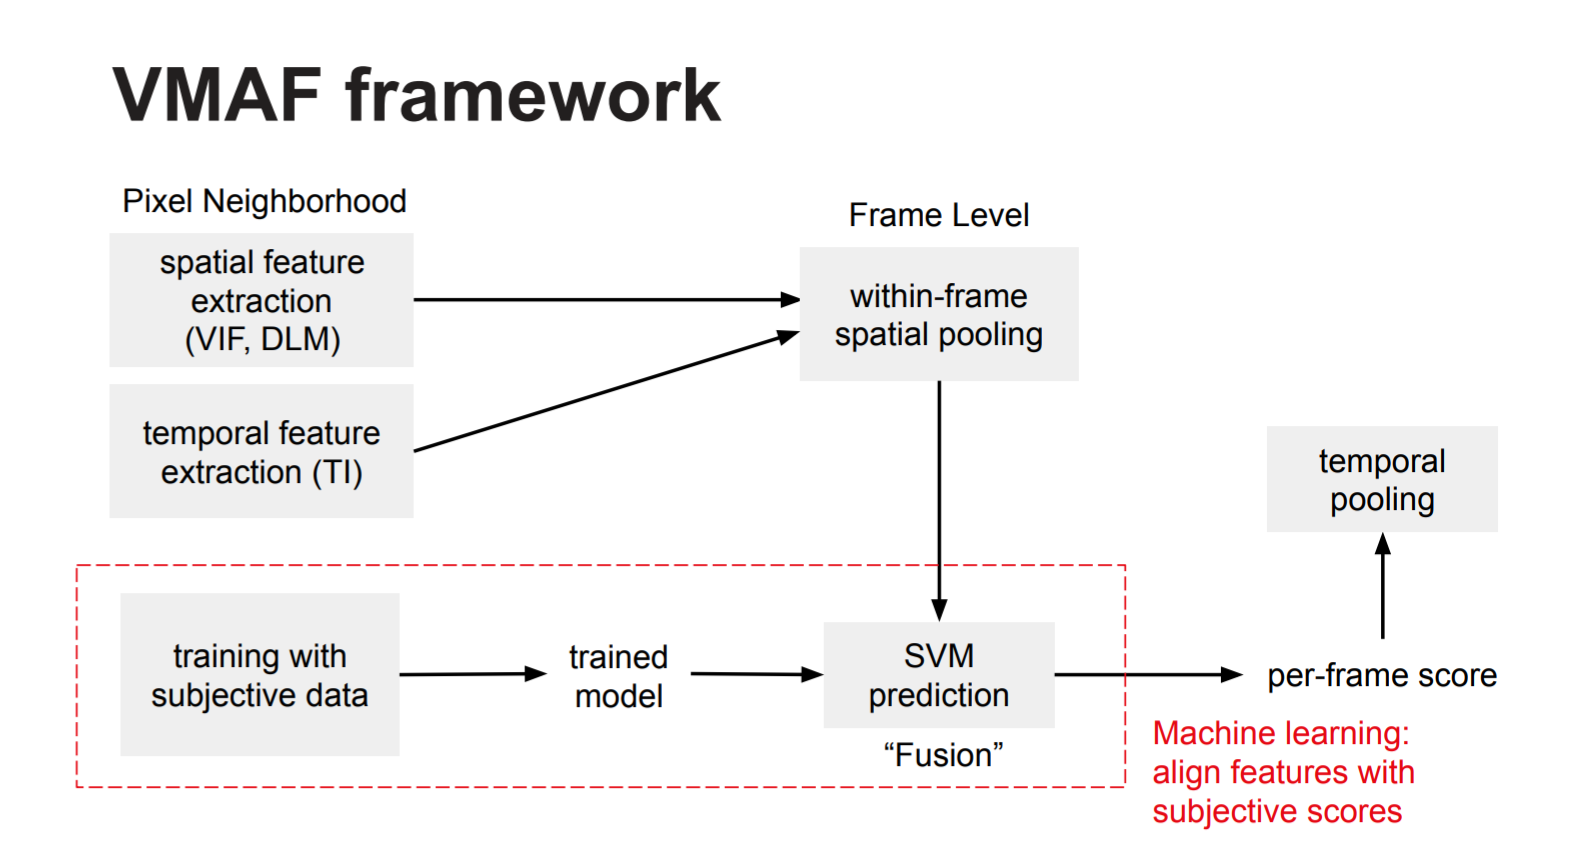
\includegraphics[width=\columnwidth]{pictures/ch4/VMAF_blk.png}
		\label{fig:VMAF_blkg}}
	\caption{Block Diagram of VMAF Framework.}\cite{bampis2018spatiotemporal}
\end{figure}

\begin{figure}[!htb]
	\begin{algorithmic}[1]
		\Function{Adaptive Video Encoding}{{\tt}}\\
		\COMMENT{\textbf{Input:} {\tt Video encoding parameters}}\\
		\COMMENT{This procedure adaptively encodes the {\tt Video stream}.}\\
		\While{ ({\textit more video GOP segments to encode})}
		
		\State{{\textbf{\textit Allocate}} Constraints and choose Optimization mode} 
		\State{\textbf{\textit Compute}} all available configs Cfg1, Cfg2 
		\State $\qquad$ {and QP ranges QP\_i and QP\_n for different GOPs}
		\State {\textbf{\textit {Combine}} Configs and QP ranges into 
			\State $\qquad$ {candidate sets C\_all and QP\_all}}
		
		\State{\textbf{\textit{Compute}} predicted objective values: 
			\State $\qquad$ {PSNR\_all, VMAF\_all, FPS\_all, Bits\_all}
			\State $\qquad$ {by applying the Forward Regression models to}
			\State $\qquad$ {candidate sets C\_all and QP\_all}}.
		
		\State{\textbf{\textit{Compute}} Pareto-front by eliminating 
			\State $\qquad$ {Points whose objectives are not }
			\State $\qquad$ {Pareto-optimal}}
		
		\State{\textbf{{\textit Find}} the Optimal encoding Parameters
			\State $\qquad$ {selecting the C\_Opt, QP\_Opt by Newton's method that}
			\State $\qquad$ {produce points that lie on the Pareto-front}
			\State $\qquad$ {candidate sets C\_all and QP\_all}}.
		
		\State{\textbf{{\textit Robust}} parameter estimation and optimization for next segment
			\State  $\qquad$  \textit{\textbf{Apply}} QP\_all and C\_all based on the current model.
			\State  $\qquad$  \textit{\textbf{Solve}} optimization problem using \textit{local search}}.
		\If {either QP\_all or C\_all is out of range}
		\State  $\qquad$ Update constraints and fix encodings
		\State  $\qquad\qquad$ new estimates of QP and Cfg
		\State  \textbf{\textit{Constrain}} QP to be within $\pm 4$ of
		\State  $\qquad\qquad$ neighboring QP ranges.
		\State  {\textbf{\textit{Enforce}} QP and Cfg within valid ranges.}
		\State { Use Previous Forward model with new estimates of QP\_all \& C\_all}	
		\EndIf
		\\~
		\State {\textbf{{\textit Encode}} the video using C\_Opt and QP\_Opt}
		\State {\textbf{{\textit Compute}} PSNR\_Opt, VMAF\_Opt, FPS\_Opt, Bits\_Opt}
		\State $\qquad$ {for current GOP segment}
		\State {\textbf{{\textit Save}} by applying the regression models to}
		\State $\qquad$ {candidate sets C\_all and QP\_all}.
		
		\EndWhile 
		\EndFunction
	\end{algorithmic}
	\caption{Overview of DRASTIC Segment based encoding framework.}
	\label{fig:Seg_enc_procedure}
\end{figure}



\begin{figure}[!hbt]
	\centering
	{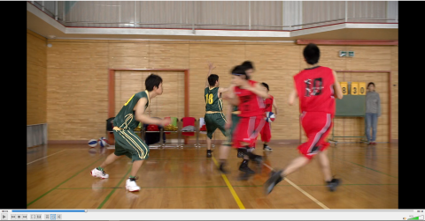
\includegraphics[width=\linewidth]{pictures/ch4/x265_1080_BasketballDrive.png}
		\label{fig:x265_BBDrive}}
	\caption{BasketballDrive from HEVC \cite{HEVCTestvideo} Video Sequence,1920x1080, 50fps.}
\end{figure}


\begin{figure}[hbt!]
	\centering
	{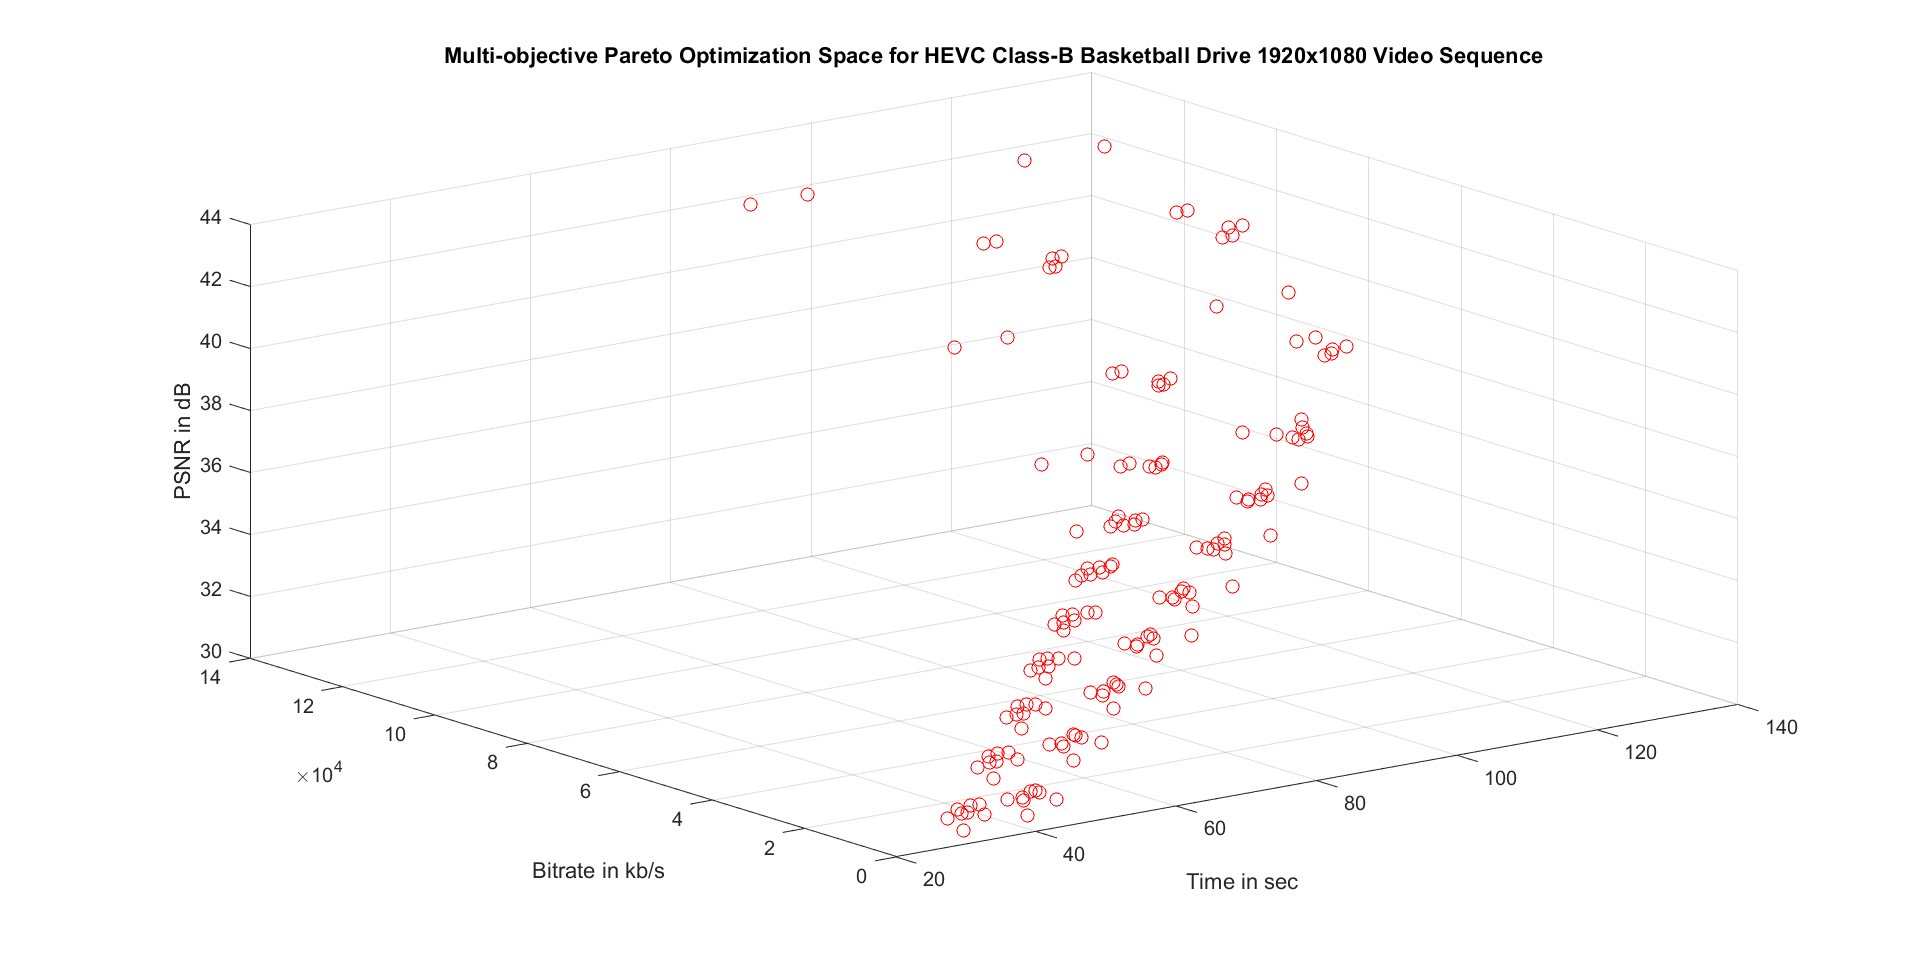
\includegraphics[width=0.8\linewidth]{pictures/ch4/BBDrive-ParetoSpace.png}
		\label{fig:BBDrive_PO}}
	\caption{Pareto Space for BasketballDrive 1920x1080, 50 fps.}
\end{figure}


\begin{figure}[hbt!]
	\centering
	{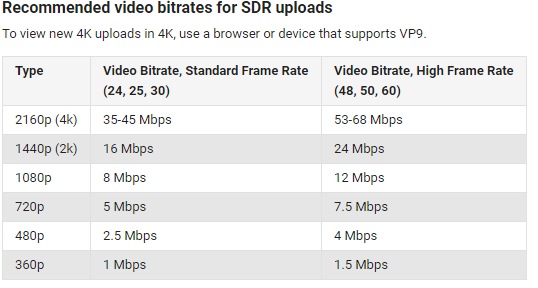
\includegraphics[width=\linewidth]{pictures/ch4/Youtube_recommendations.png}
		\label{fig:YouTube_Bitrates}}
	\caption{YouTube Recommended Bitrates for different resolutions \cite{YouTube}.}
\end{figure}



\begin{figure}[hbt!]
	\centering
	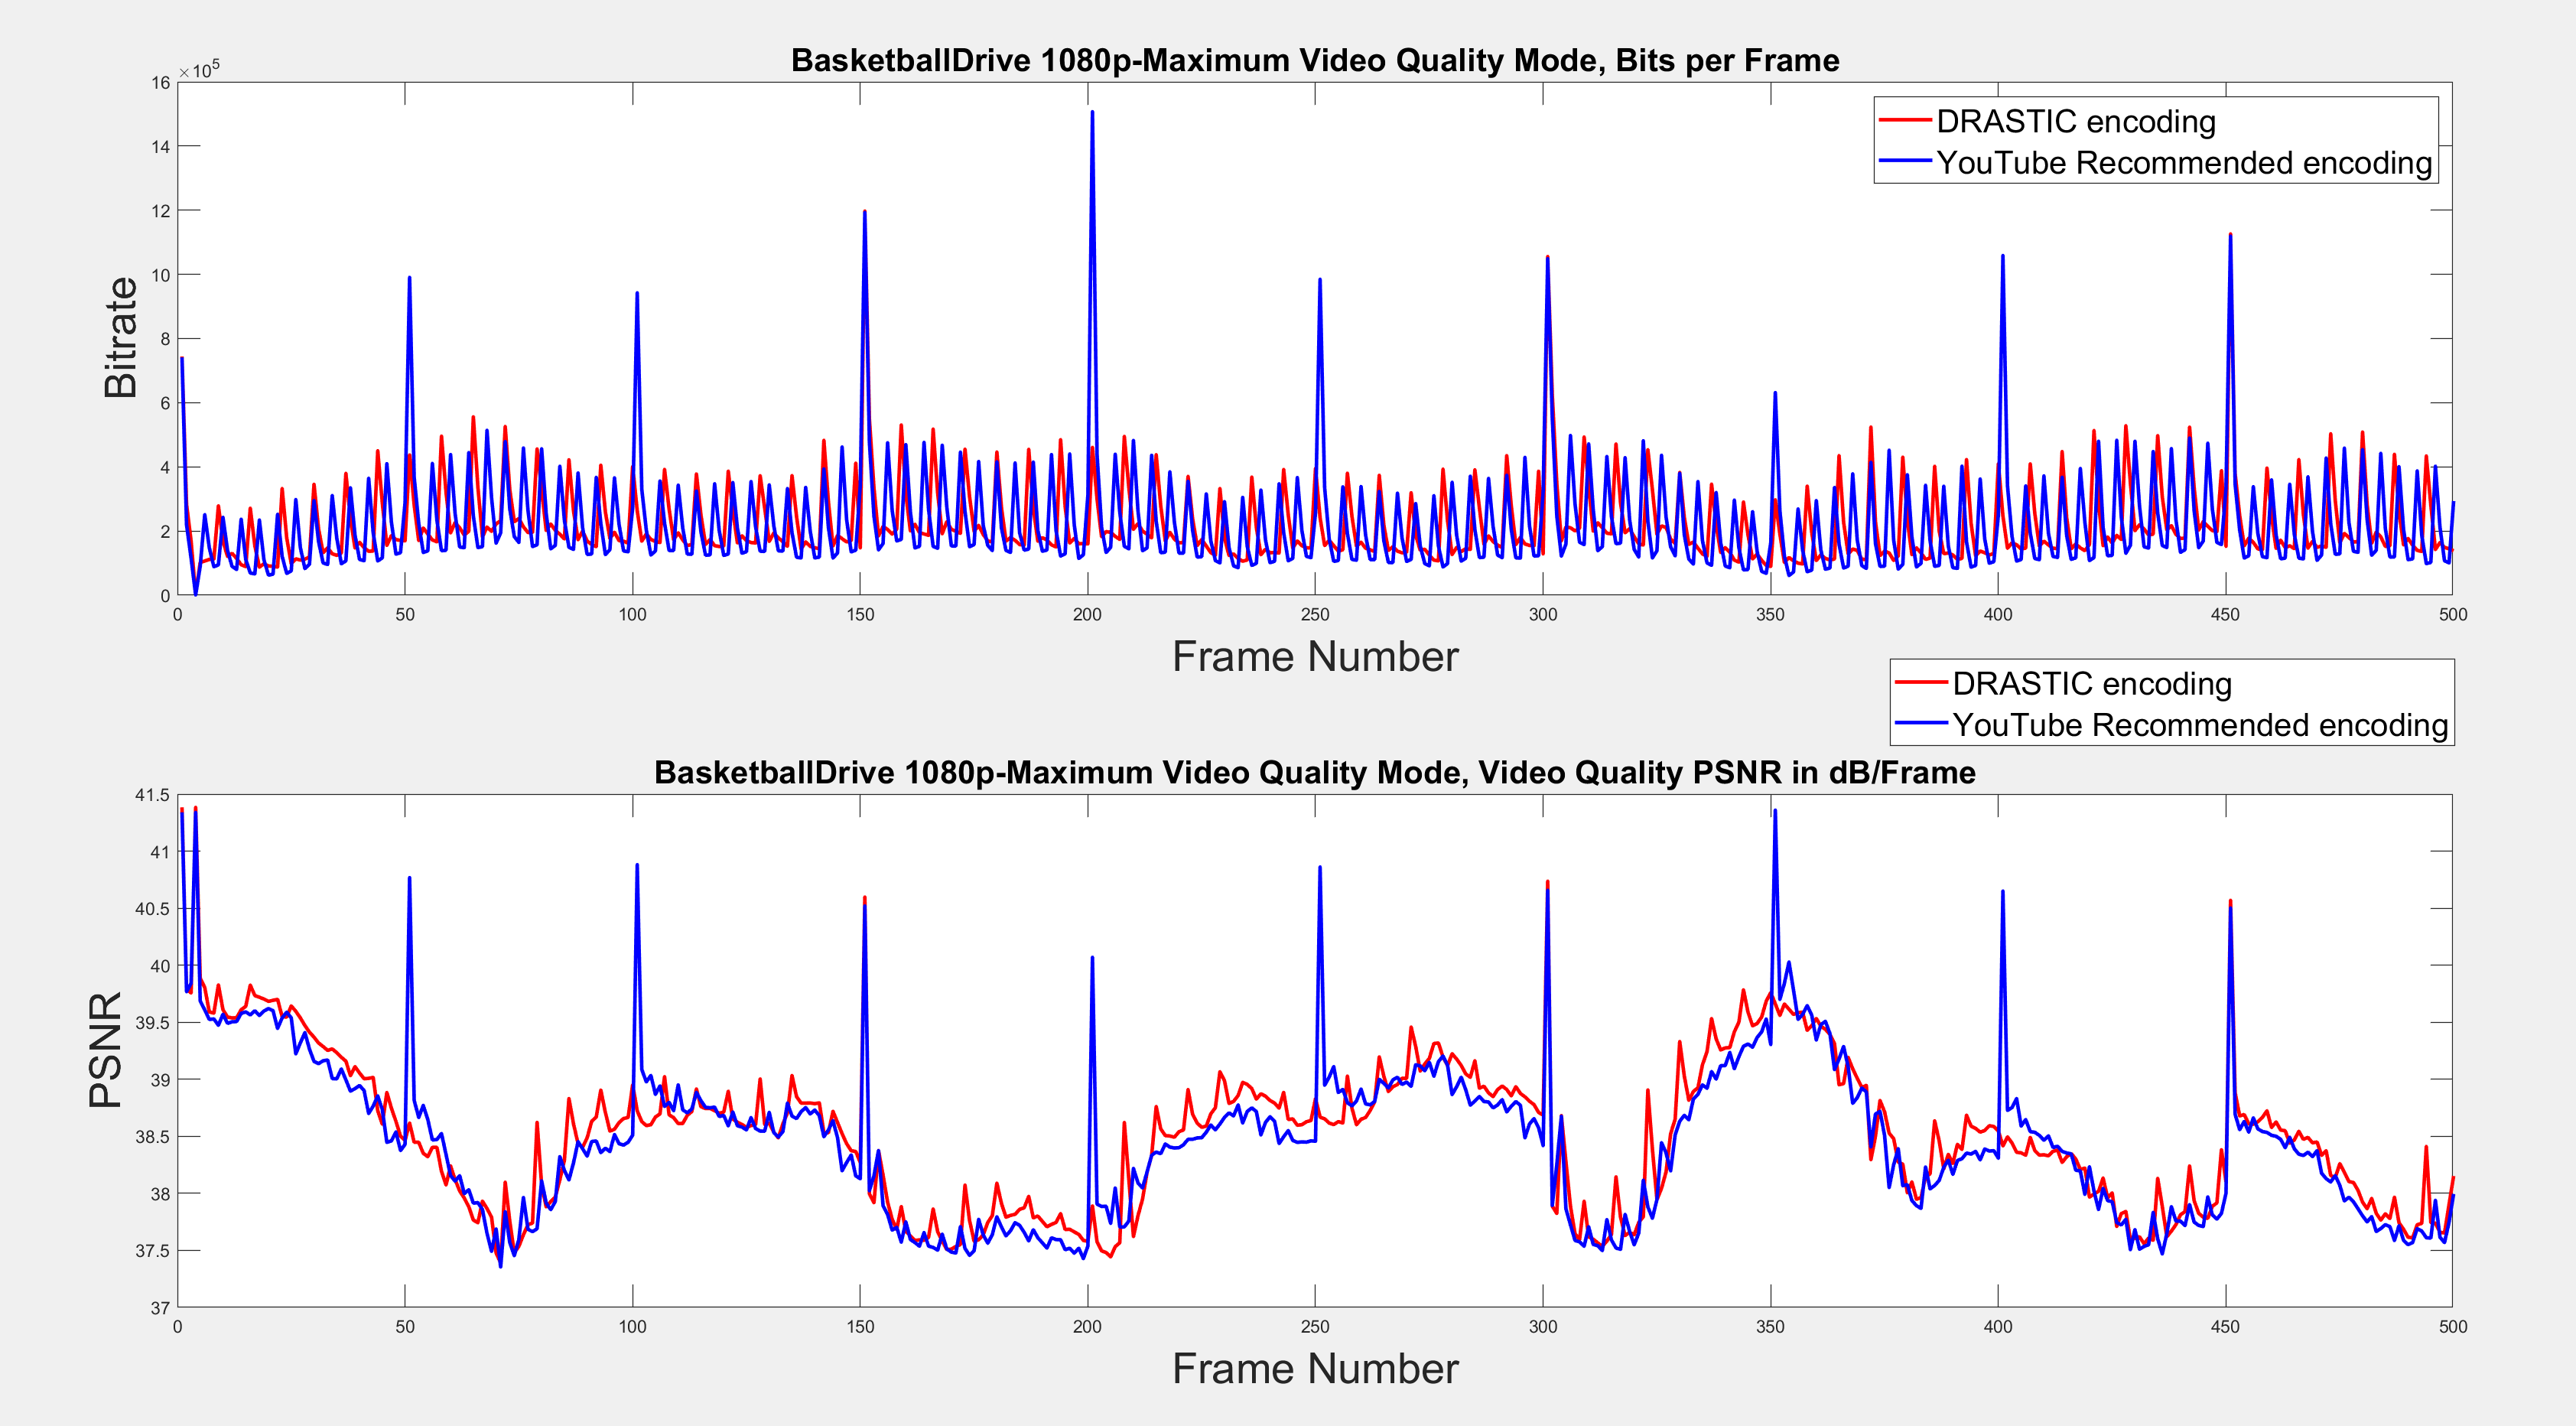
\includegraphics[width=\linewidth]{pictures/ch4/BBDrive_MaxQ.png}
	\caption{HEVC Test sequence, 1920x1080, BasketballDrive maximum Quality Mode.}
	\label{fig:BBDrive_maxQ}
\end{figure}





\begin{figure}[hbt!]
	\centering
	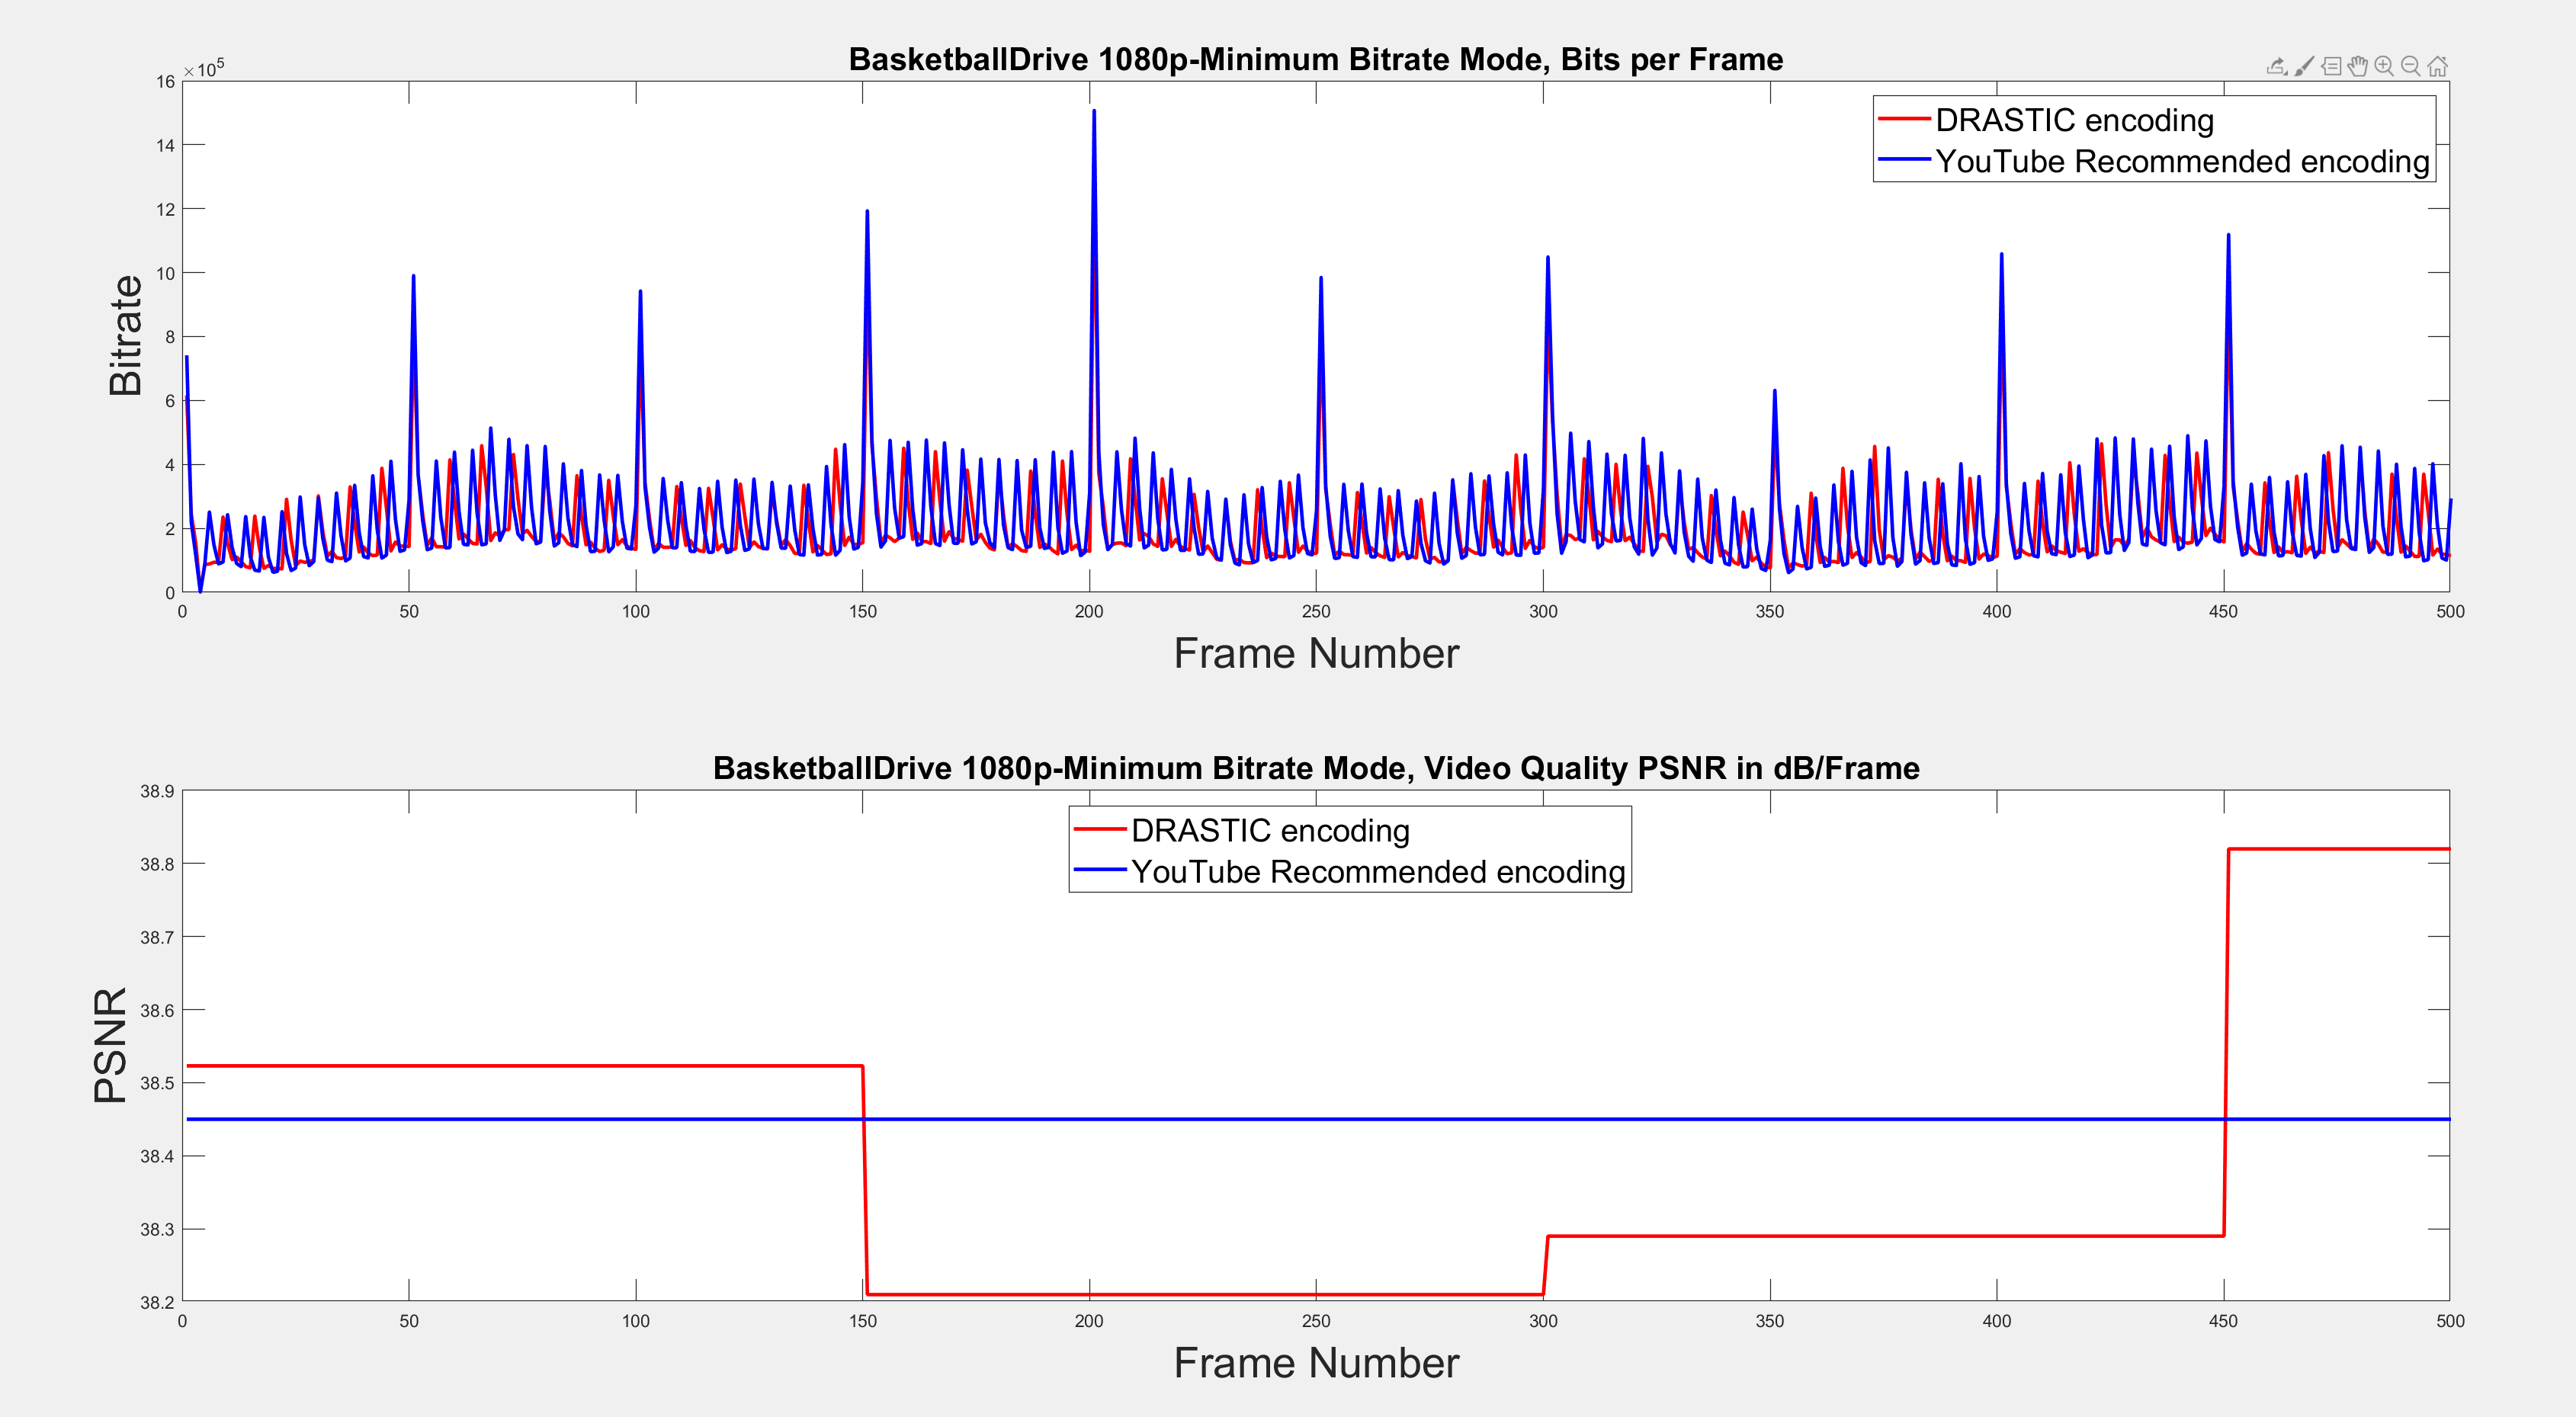
\includegraphics[width=\linewidth]{pictures/ch4/BBDrive_MinBits1.png}
	\caption{HEVC Test sequence, 1920x1080, BasketballDrive minimum Bitrate Mode.}
	\label{fig:BBDrive_minB}
\end{figure}

\begin{figure}[hbt!]
	\centering
	{\includegraphics[width=\linewidth]{pictures/ch4/Cactus_1080p.png}
		\label{fig:x265_Cactus}}
	\caption{Cactus from HEVC \cite{HEVCTestvideo} Video Sequence,1920x1080, 50fps.}
\end{figure}

\begin{figure}[hbt!]
	\centering
	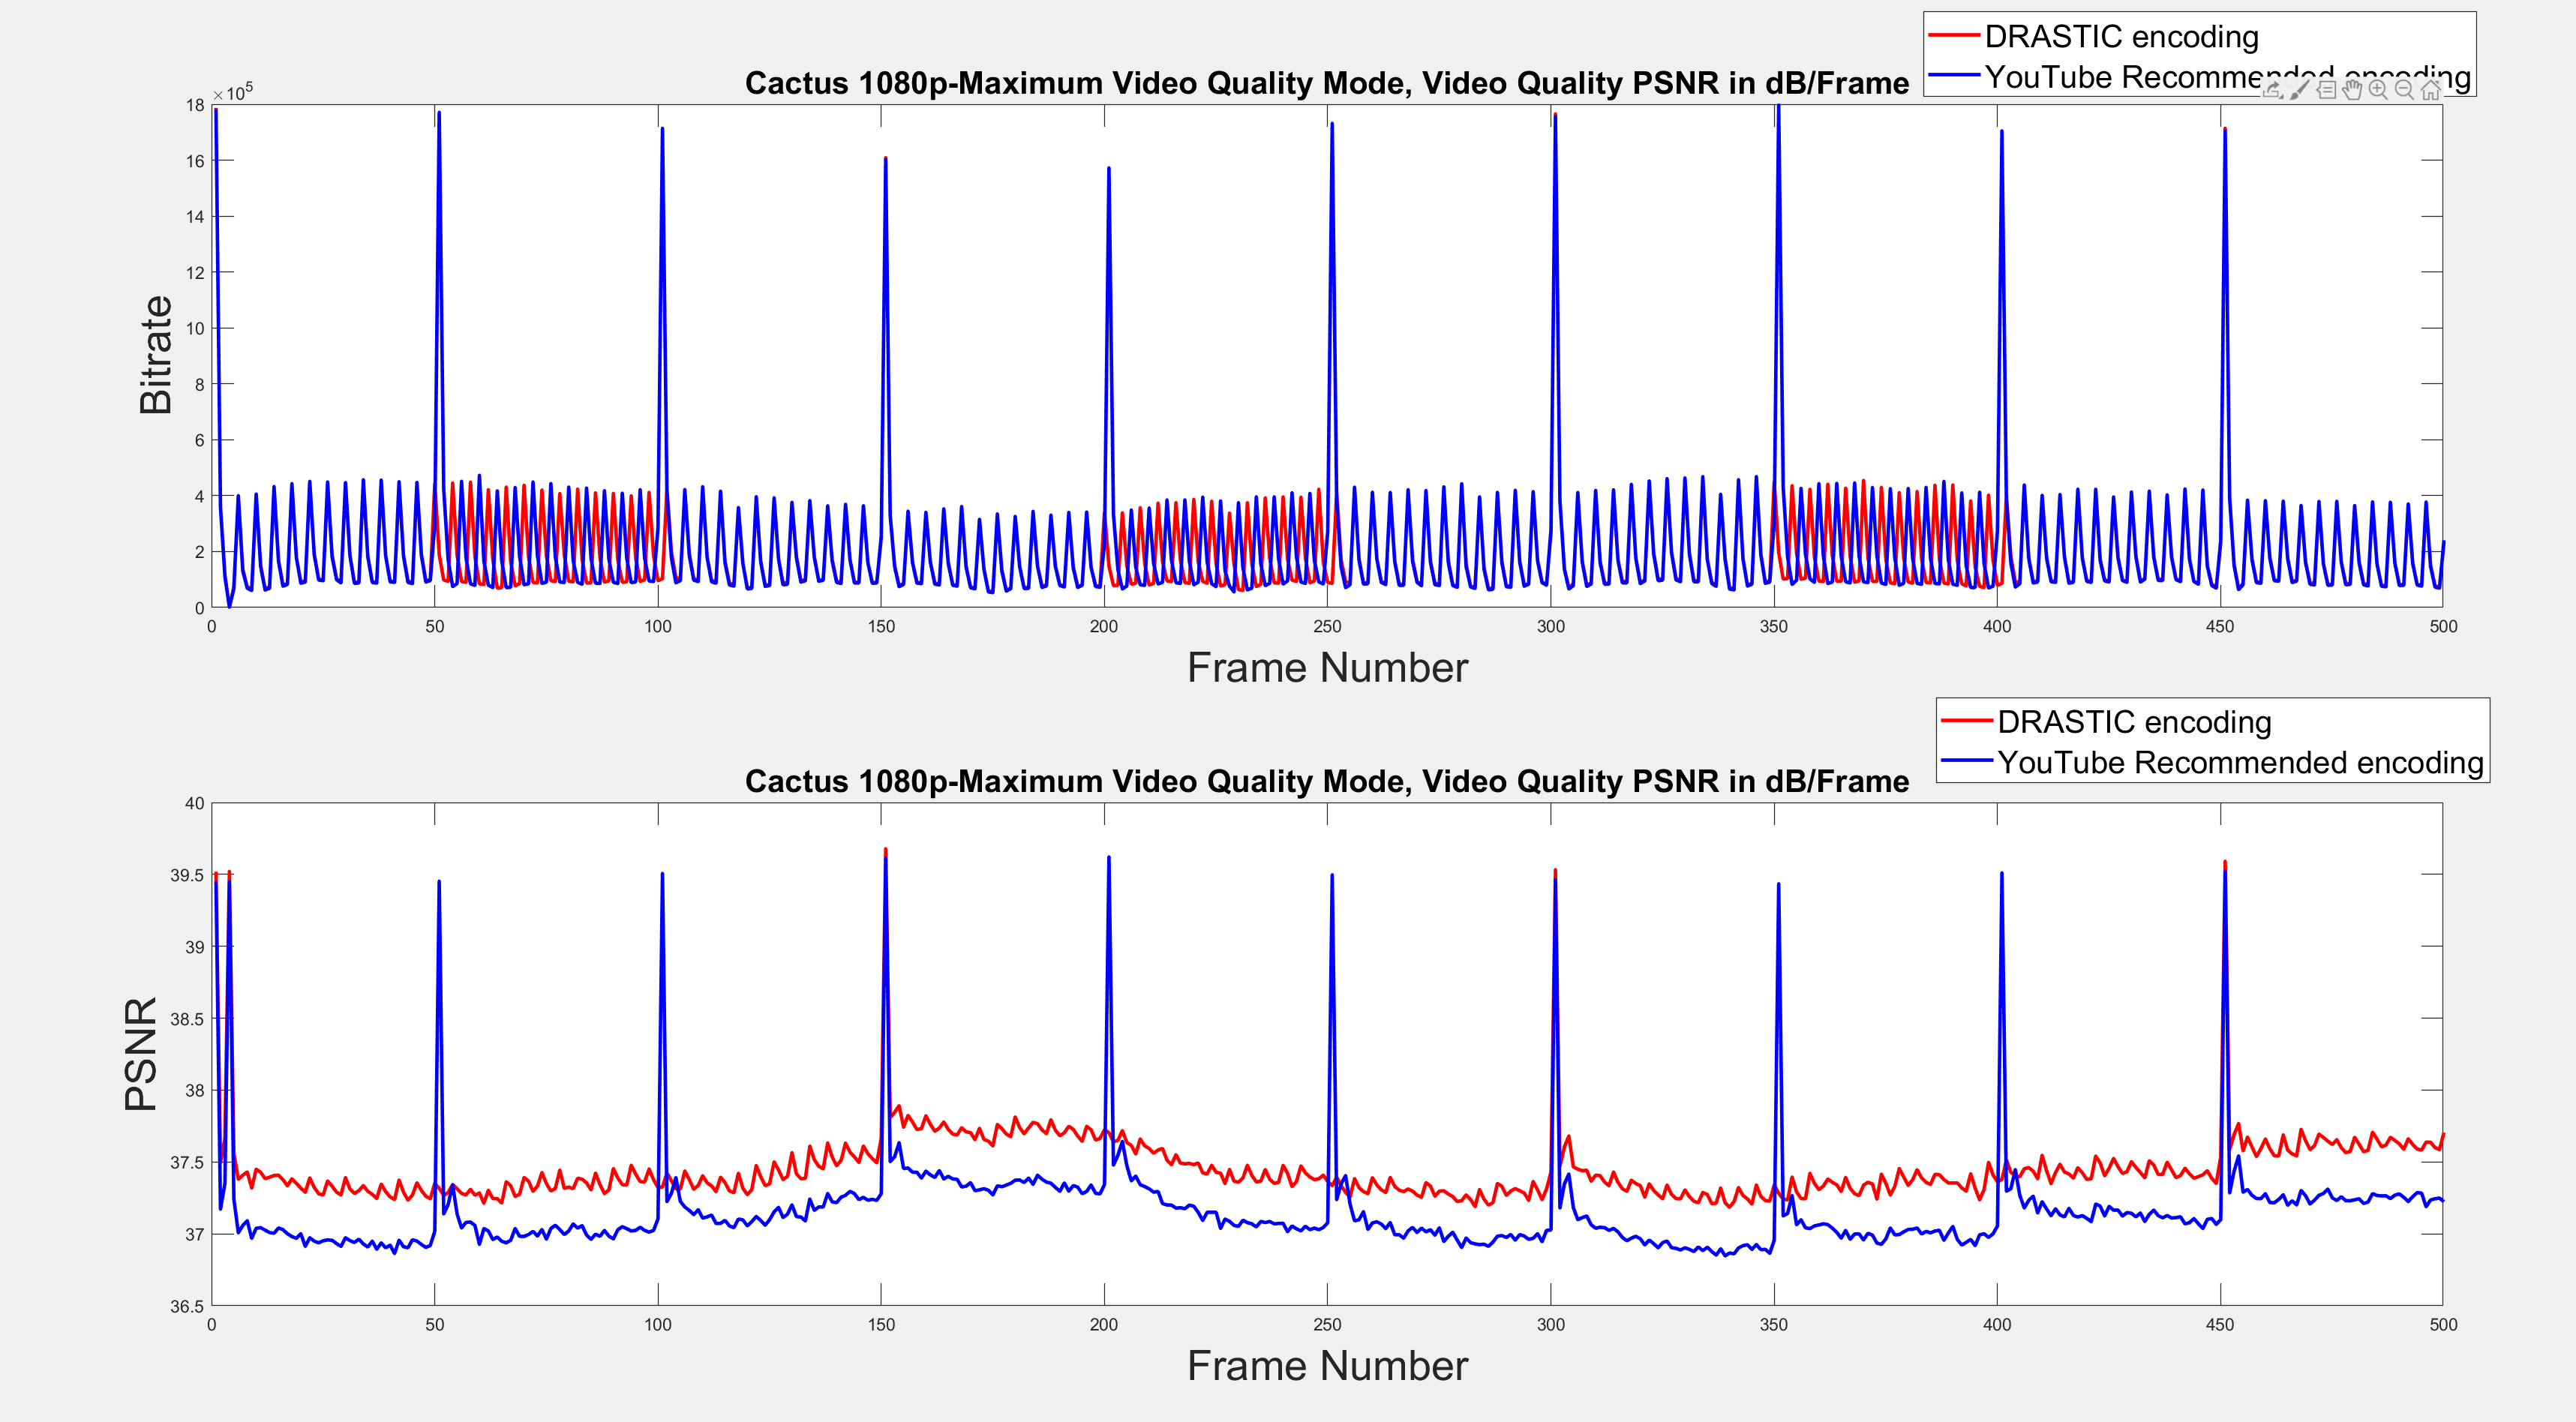
\includegraphics[width=\linewidth]{pictures/ch4/Cactus_MaxQ.png}
	\caption{HEVC Test sequence, 1920x1080, Cactus Maximum Video Quality Mode.}
	\label{fig:Cactus_maxQ}
\end{figure}

\begin{figure}[hbt!]
	\centering
	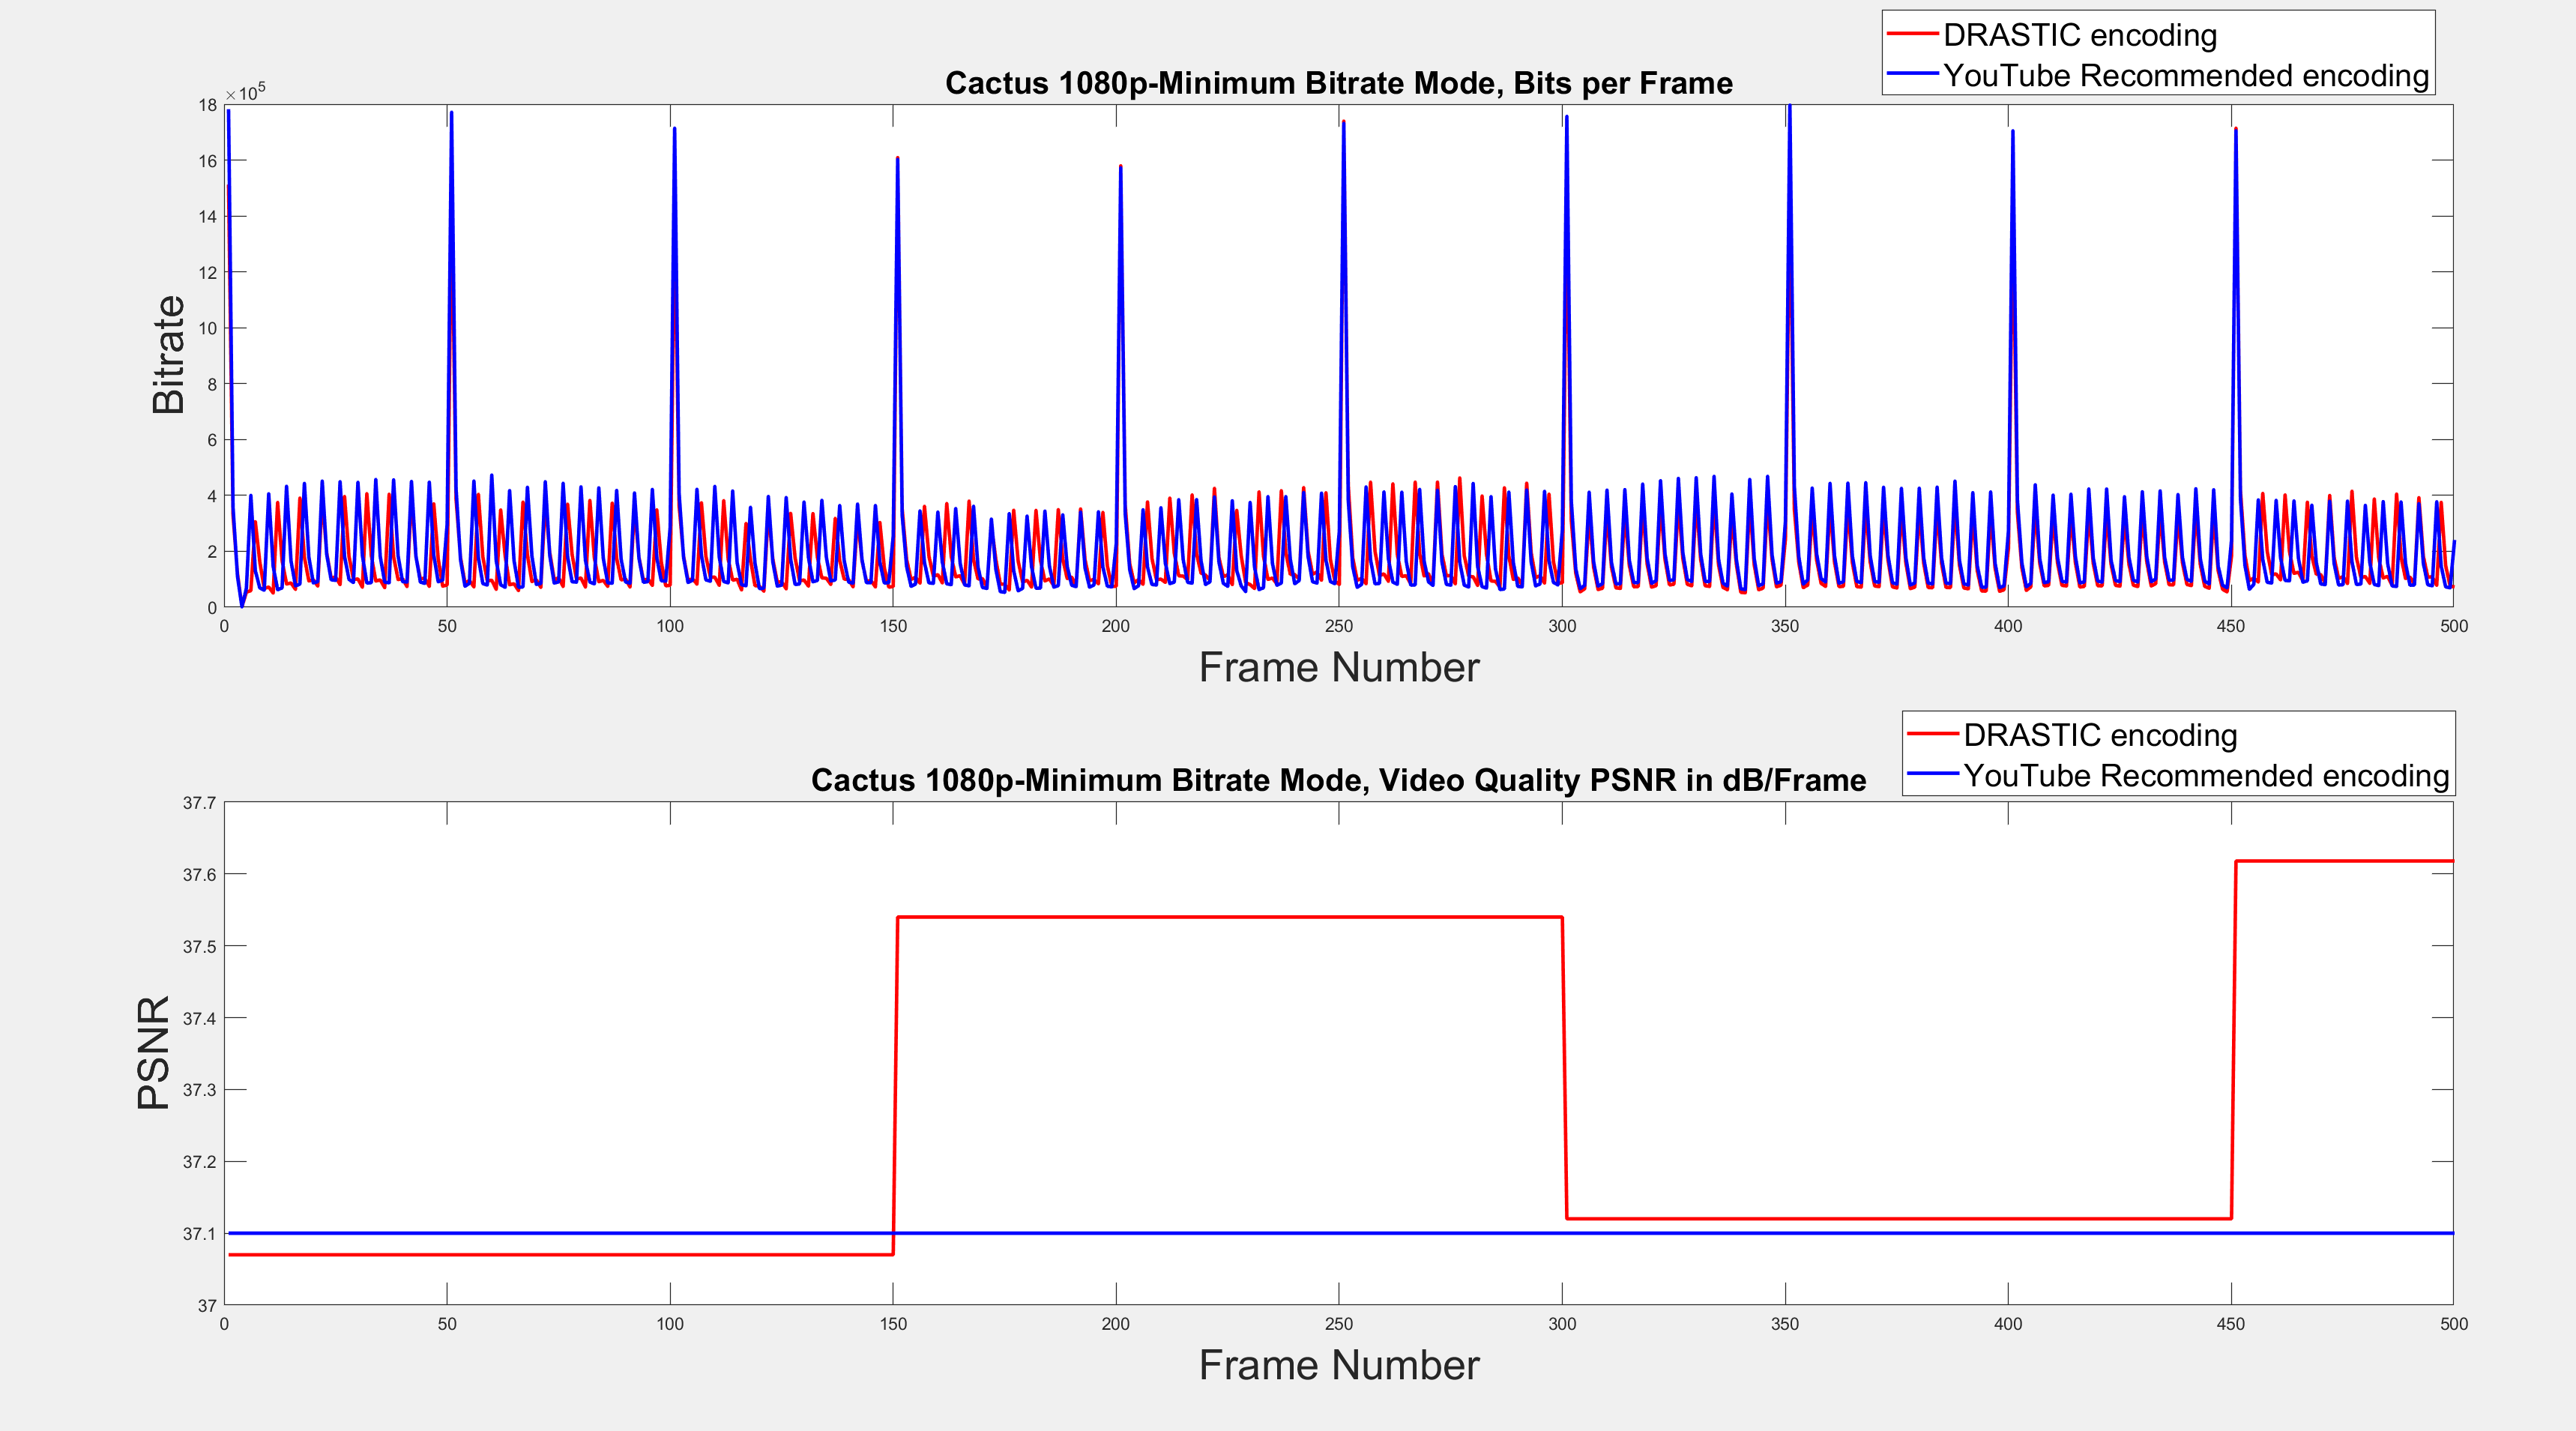
\includegraphics[width=\linewidth]{pictures/ch4/Cactus_MinB.png}
	\caption{HEVC Test sequence, 1920x1080, Cactus Minimum Bitrate Mode.}
	\label{fig:Cactus_minBits}
\end{figure}


%
%                                       Chpater 5
%
\chapter[Overview of Google VP9 Codec for VoD]{Overview of Google VP9 Codec with Segment based encoding at GOP level}


\begin{figure}[hbt!]
	\centering
	{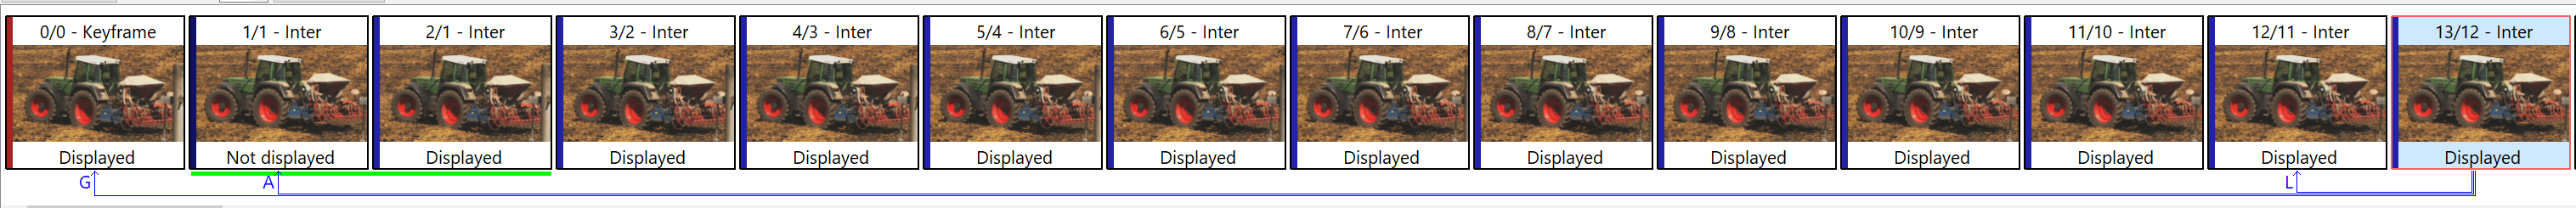
\includegraphics[width=\columnwidth]{pictures/ch5/VP9_GOP_Bitstream_visual.png}
		\label{fig:GOPs-in-Bitstream}}
	\caption{VP9 GOPs in WebM bitstream}
\end{figure}
\begin{figure}[hbt!]
	\centering
	\subfloat[VP9 GOP with AltRef 1]
	{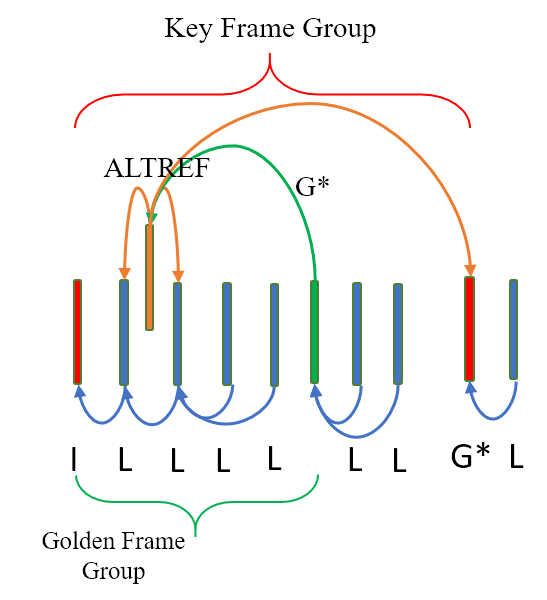
\includegraphics[width=0.5\textwidth]{pictures/ch5/VP9_ALT1_GOP.png}
		\label{fig:VP9_ALT1_GOP}}
	\subfloat[VP9 GOP with AltRef 2]
	{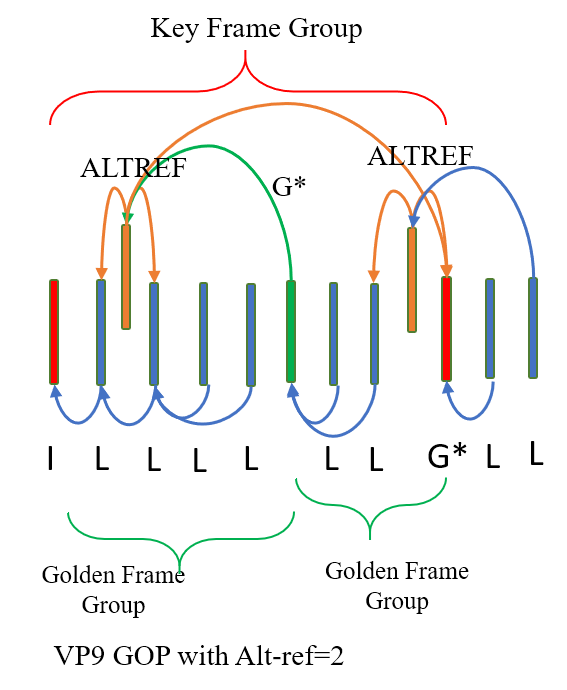
\includegraphics[width=0.4\textwidth]{pictures/ch5/VP9_ALT2_GOP.png}
		\label{fig:VP9_ALT2_GOP}} \\

	\caption{VP9 GOP Structures with Golden Frame Groups
		(a) Alternate Reference \textbf{AltRef1} frame.
		(b) Alternate Reference \textbf{AltRef2} frame.}     
	\label{fig:VP9GOPs}
\end{figure}

\begin{figure}[hbt!]
	\centering
	{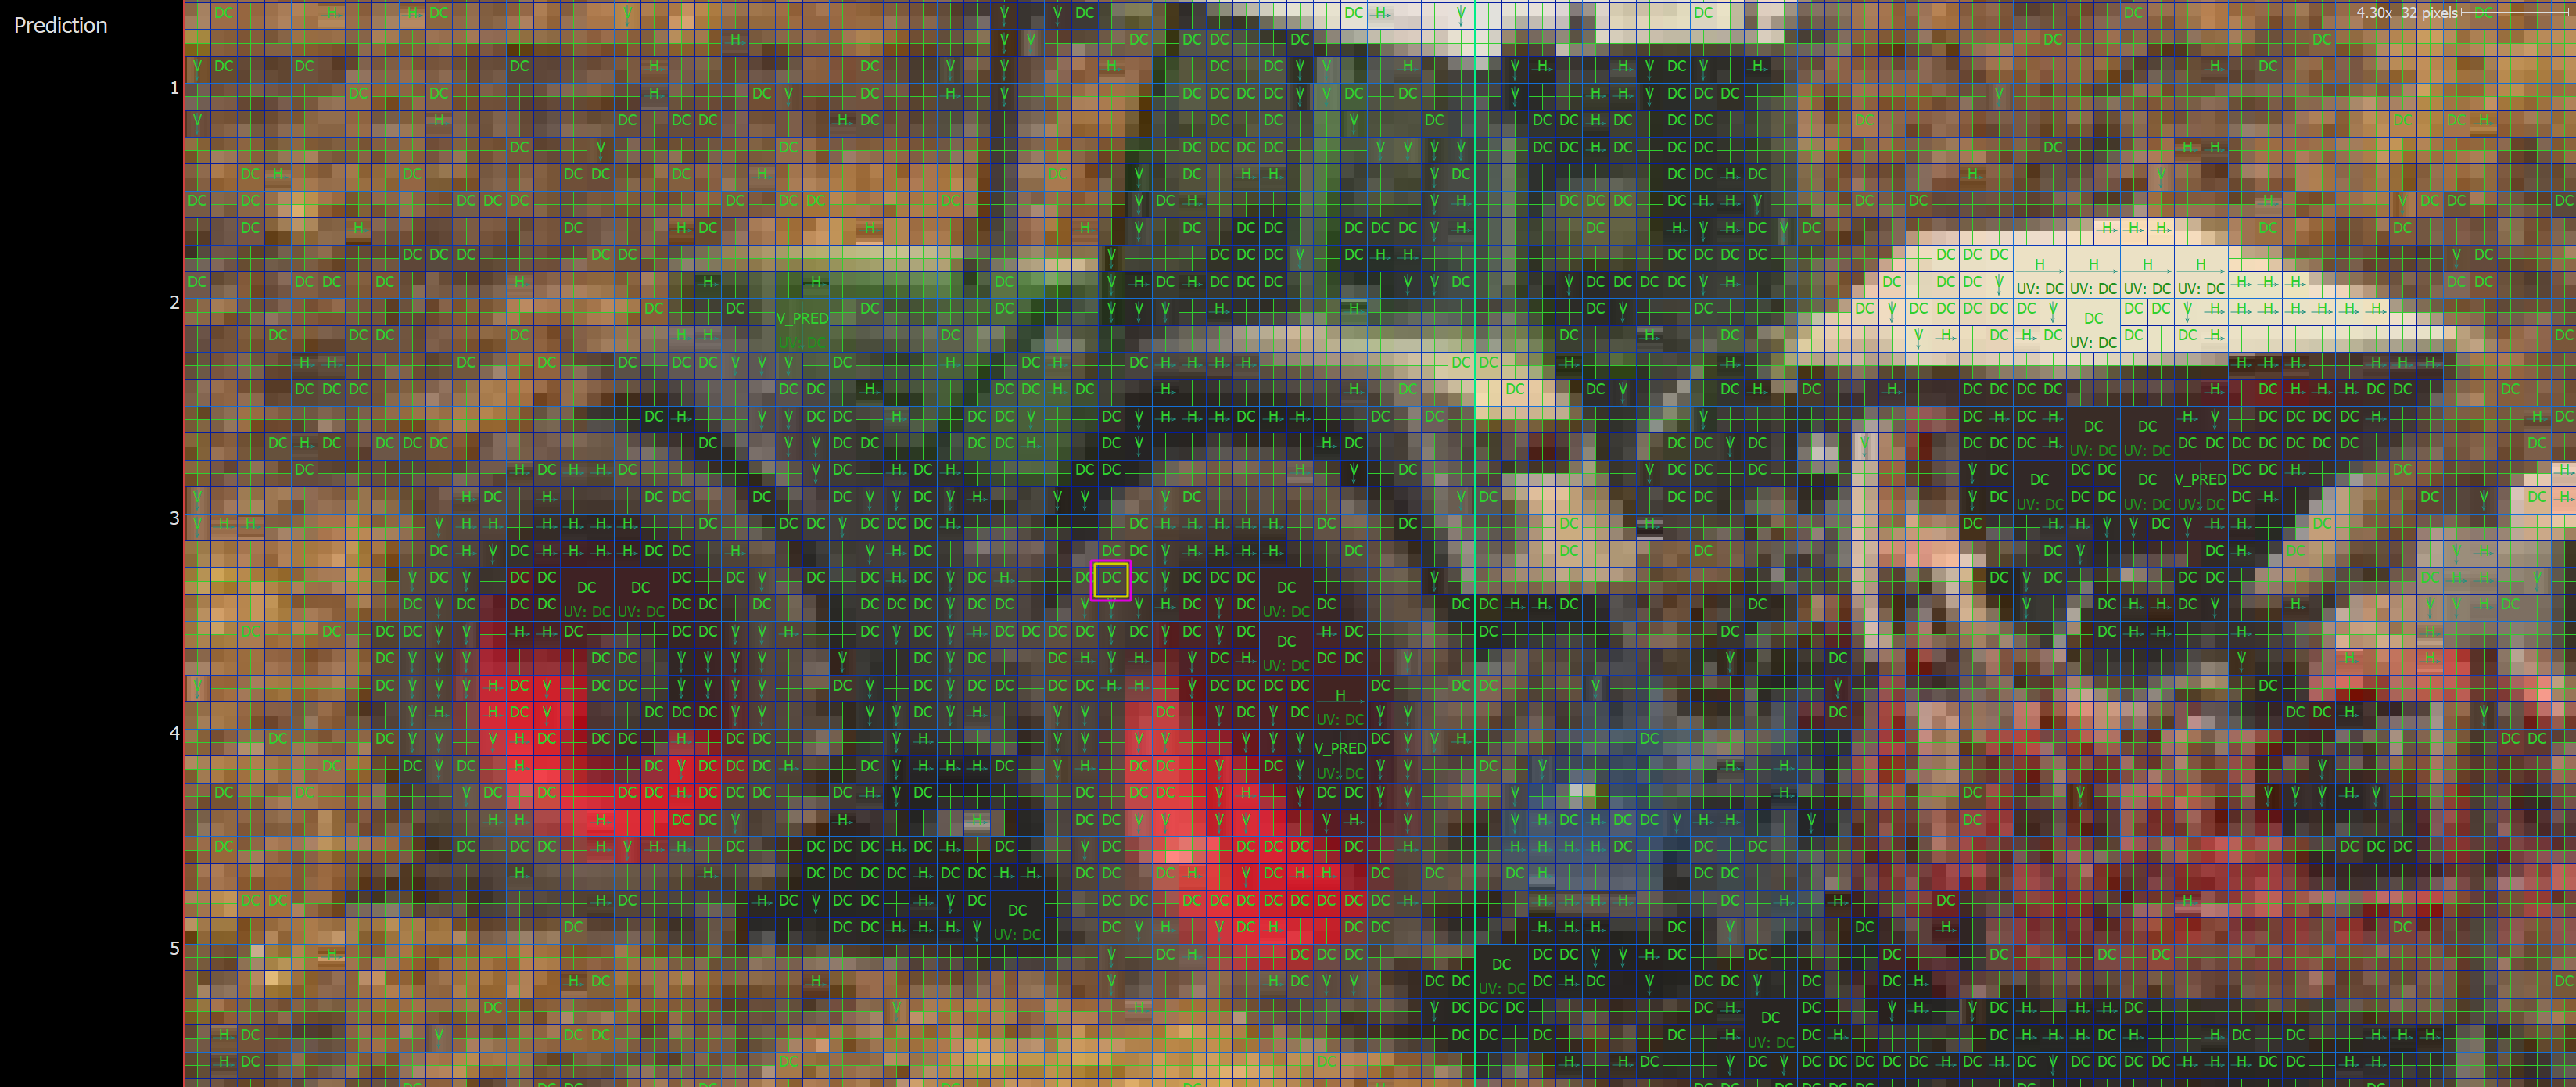
\includegraphics[width=\columnwidth]{pictures/ch5/VP9-IntraModes.png}
		\label{fig:VP9-IntraModes}}
	\caption{VP9 Intra modes.}
\end{figure}
\begin{figure}[hbt!]
	\centering
	{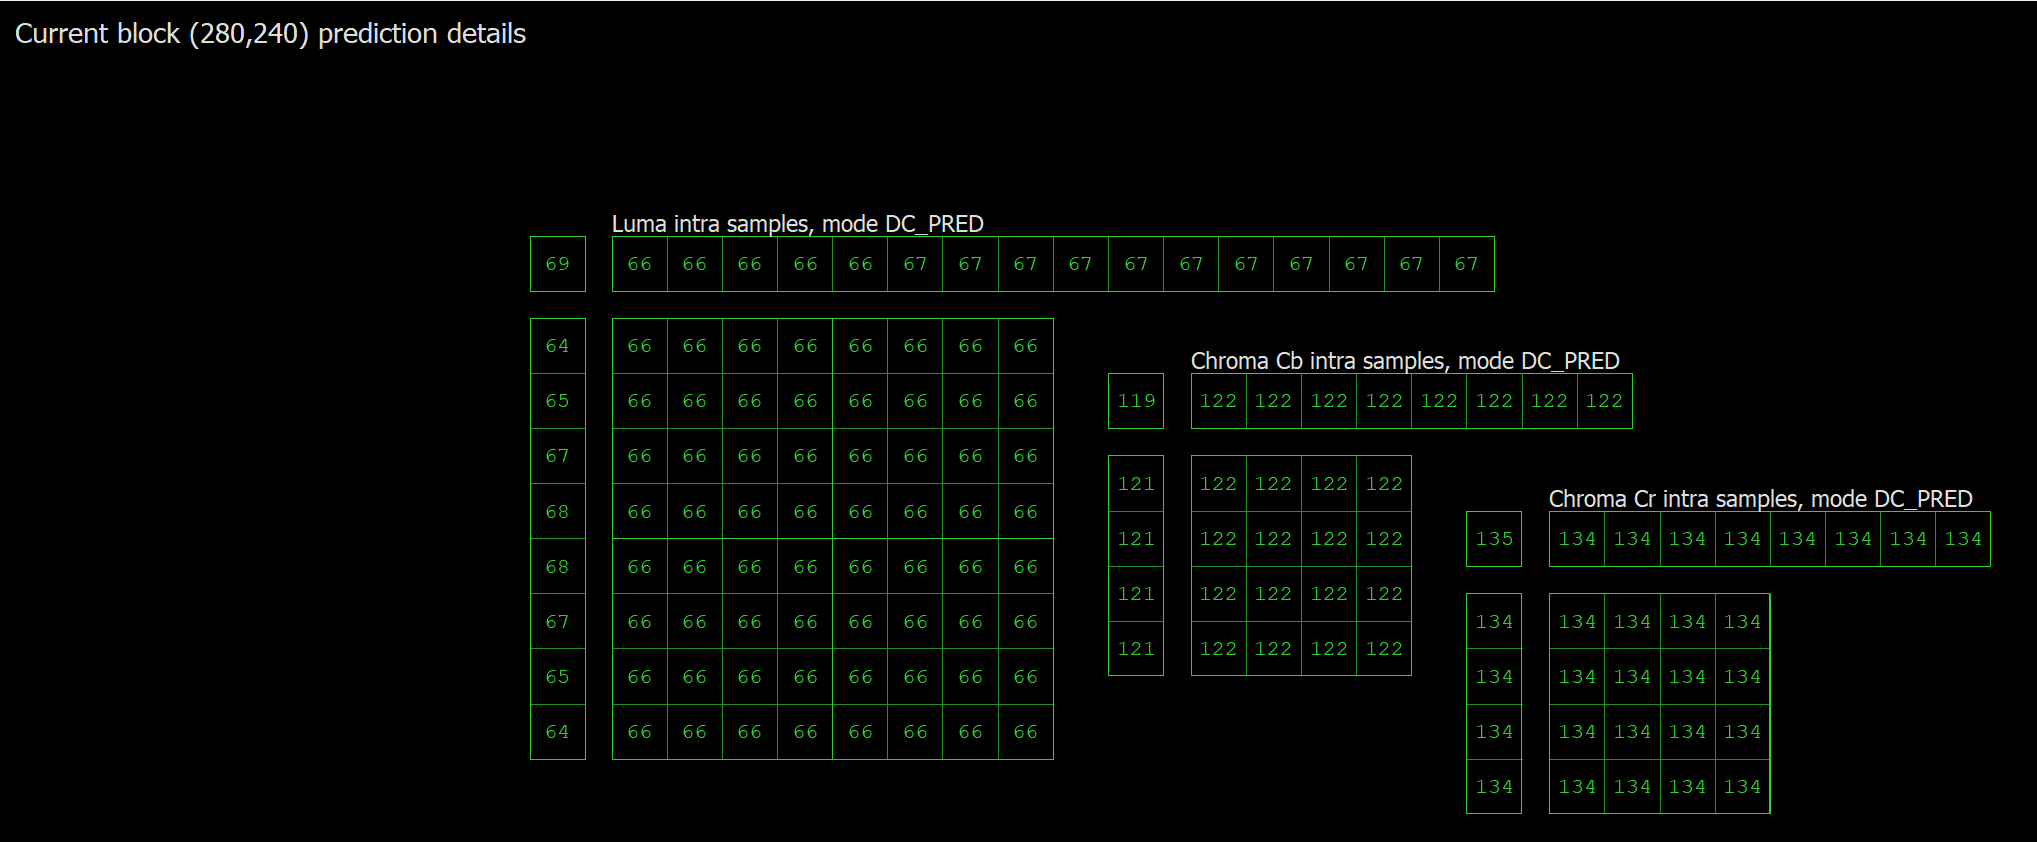
\includegraphics[width=\columnwidth]{pictures/ch5/VP9-Intra-Mode-Detail.png}
		\label{fig:VP9-IntraModes-Detail}}
	\caption{VP9 Intra prediction with Luma and Chroma in DC Mode.}
\end{figure} 

\begin{figure}[hbt!]
	\centering
	{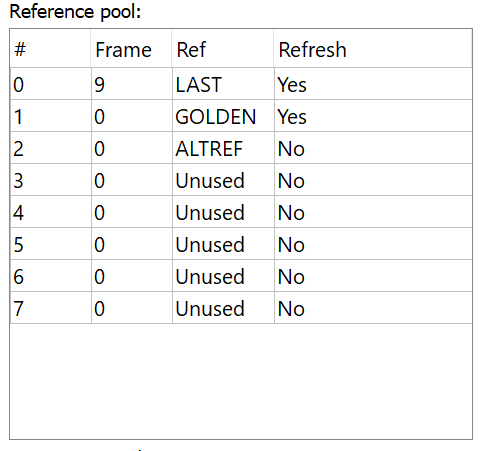
\includegraphics[width=1.9 true in]{pictures/ch5/VP9-Ref-pool.png}
		\label{fig:VP9-Refpool}}
	\caption{VP9 reference pool of frames.}
\end{figure}


\begin{figure}[hbt!]
	\centering
	{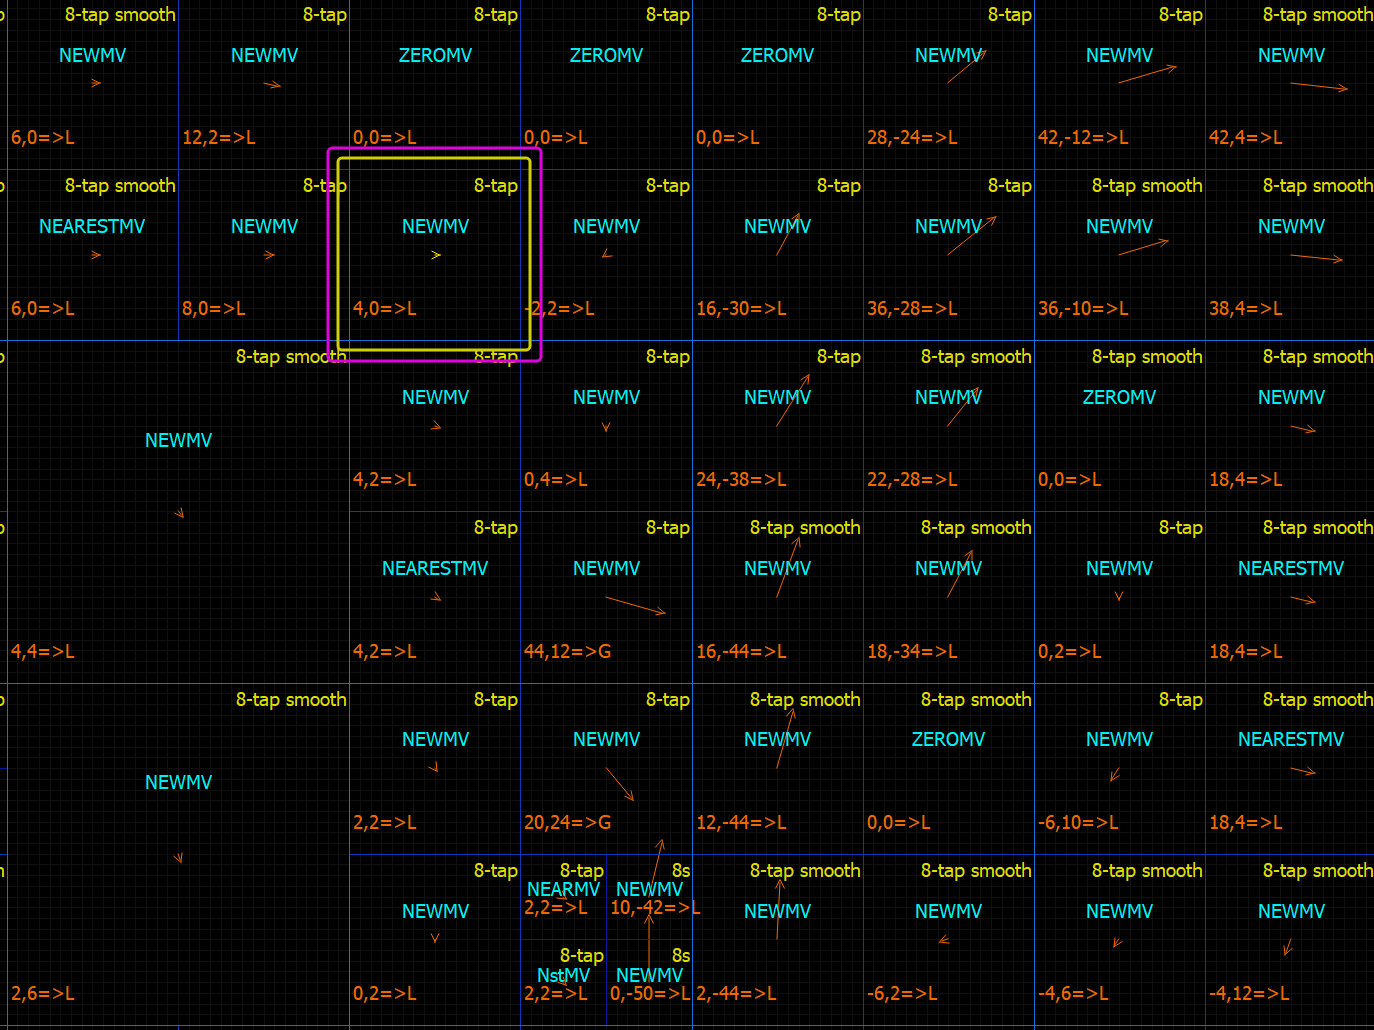
\includegraphics[width=\columnwidth]{pictures/ch5/VP9-MVs.png}
		\label{fig:VP9-MVs}}
	\caption{VP9 Motion Vectors.}
\end{figure}



\begin{figure}[h!]
	\centering
	{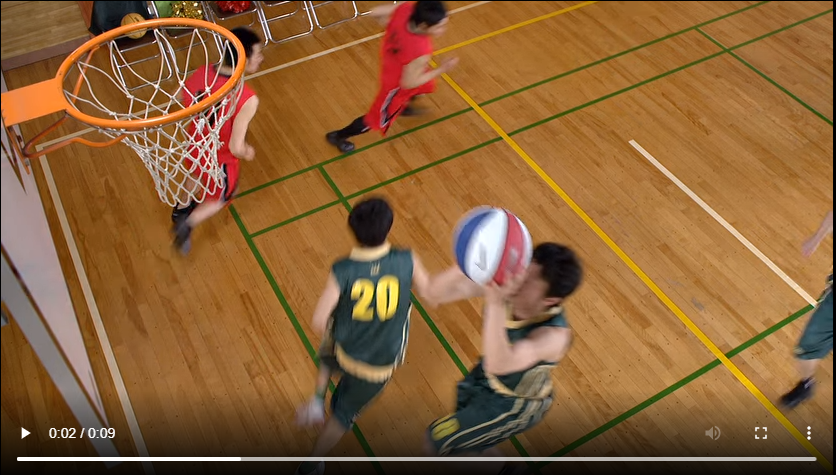
\includegraphics[width=\columnwidth]{pictures/ch5/BasketballDrill_VP9.png}
		\label{fig:Vp9_BBDrill}}
	\caption{BasketballDrill from HEVC \cite{HEVCTestvideo} Video Sequence, 832x480, 50fps.}
\end{figure}

%
%                                       Chpater 6
%
\chapter[SVT-AV1: A Scalable, Open Source AV1 Codec and Pareto Models]{SVT-AV1: A Scalable, Open Source AV1 Codec and Local Pareto Models at GOP level}


\begin{figure}[hbt!]
	\centering
	{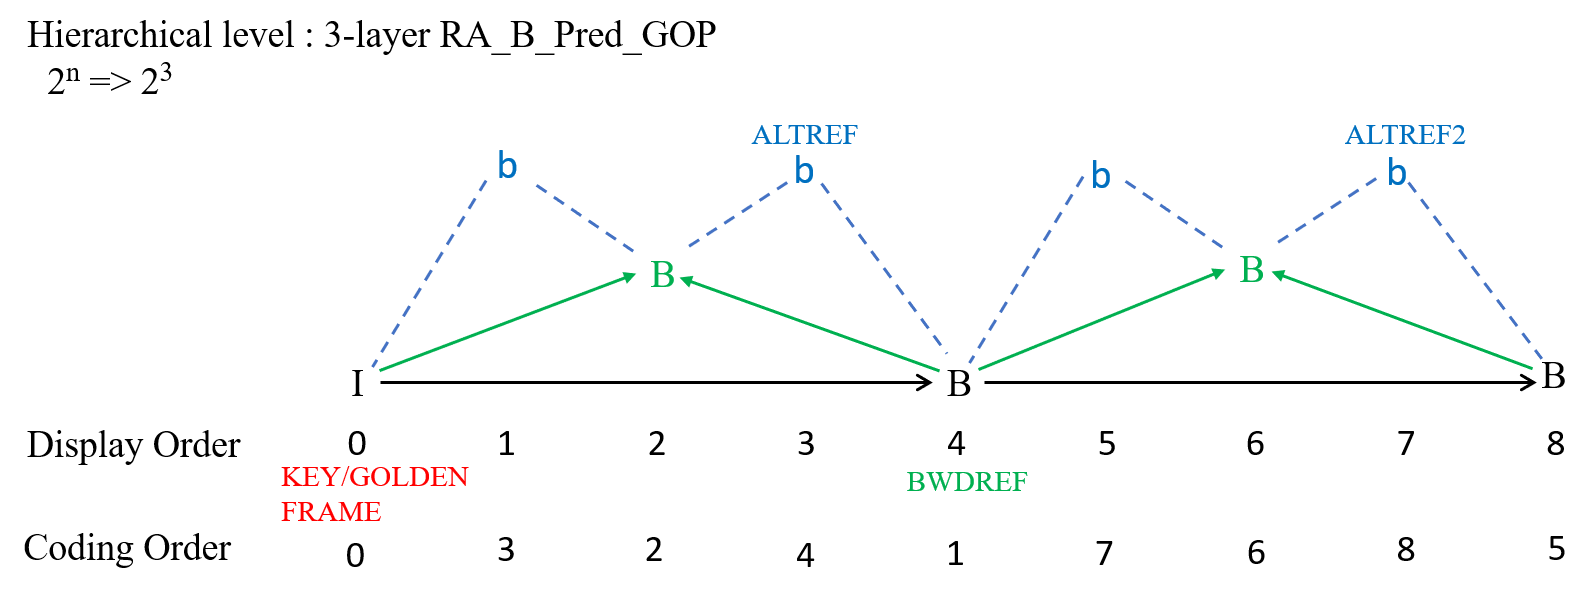
\includegraphics[width=\columnwidth]{pictures/ch6/SVT-AV1_HL3_GOP.png}
		\label{fig:SVT-AV1-HL3}}
	\caption{Hierarchical GOP Structure HL3 of SVT-AV1} \cite{SVTAV1design}
\end{figure}

\begin{figure}[hbt!]
	\centering
	{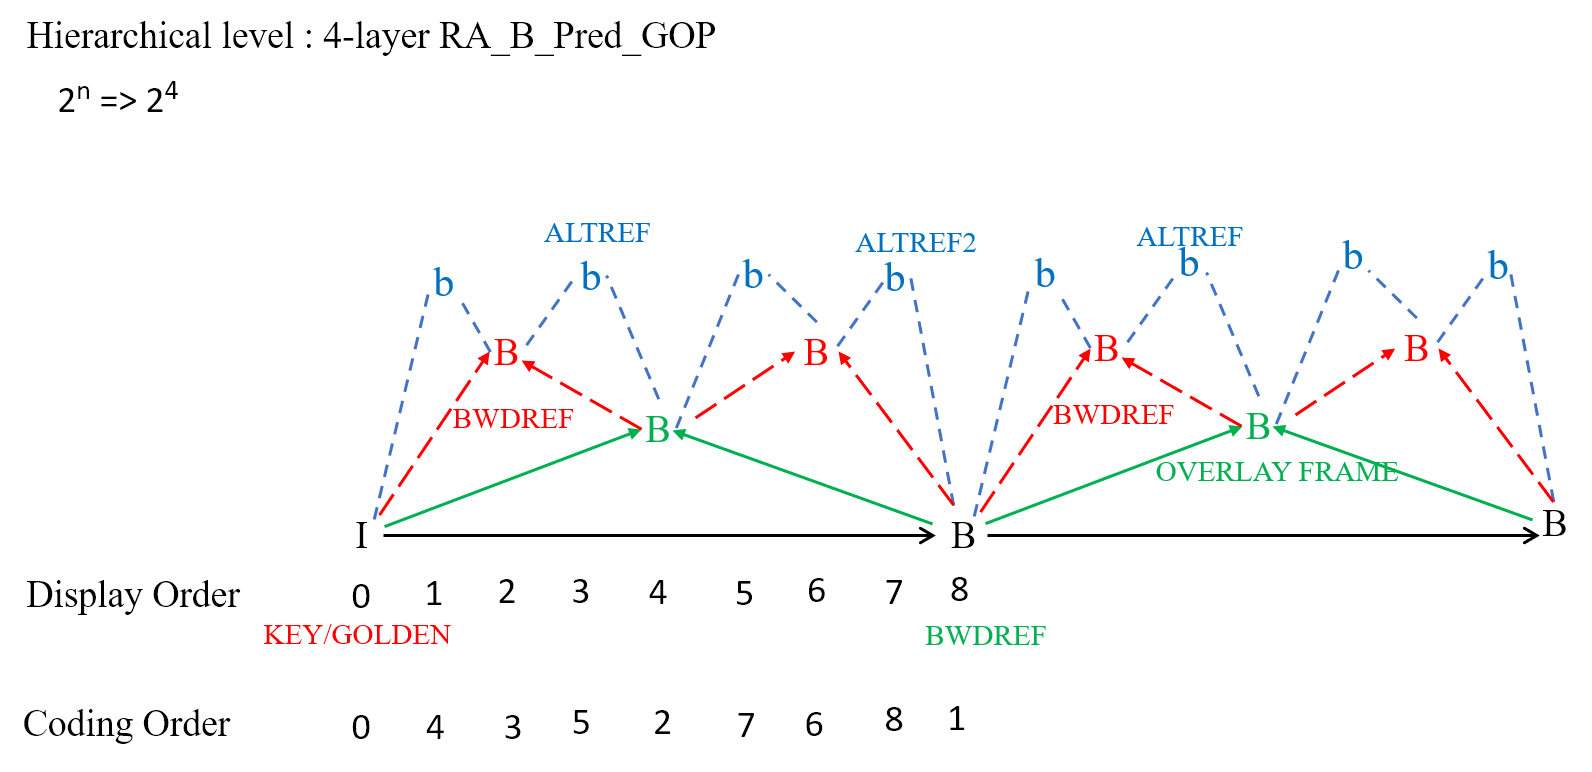
\includegraphics[width=\columnwidth]{pictures/ch6/SVT-AV1_HL4_GOP.png}
		\label{fig:SVT-AV1-HL4}}
	\caption{Hierarchical GOP Structure HL4 of SVT-AV1} \cite{SVTAV1design}
\end{figure}


\begin{figure}[h!]
	\centering
	{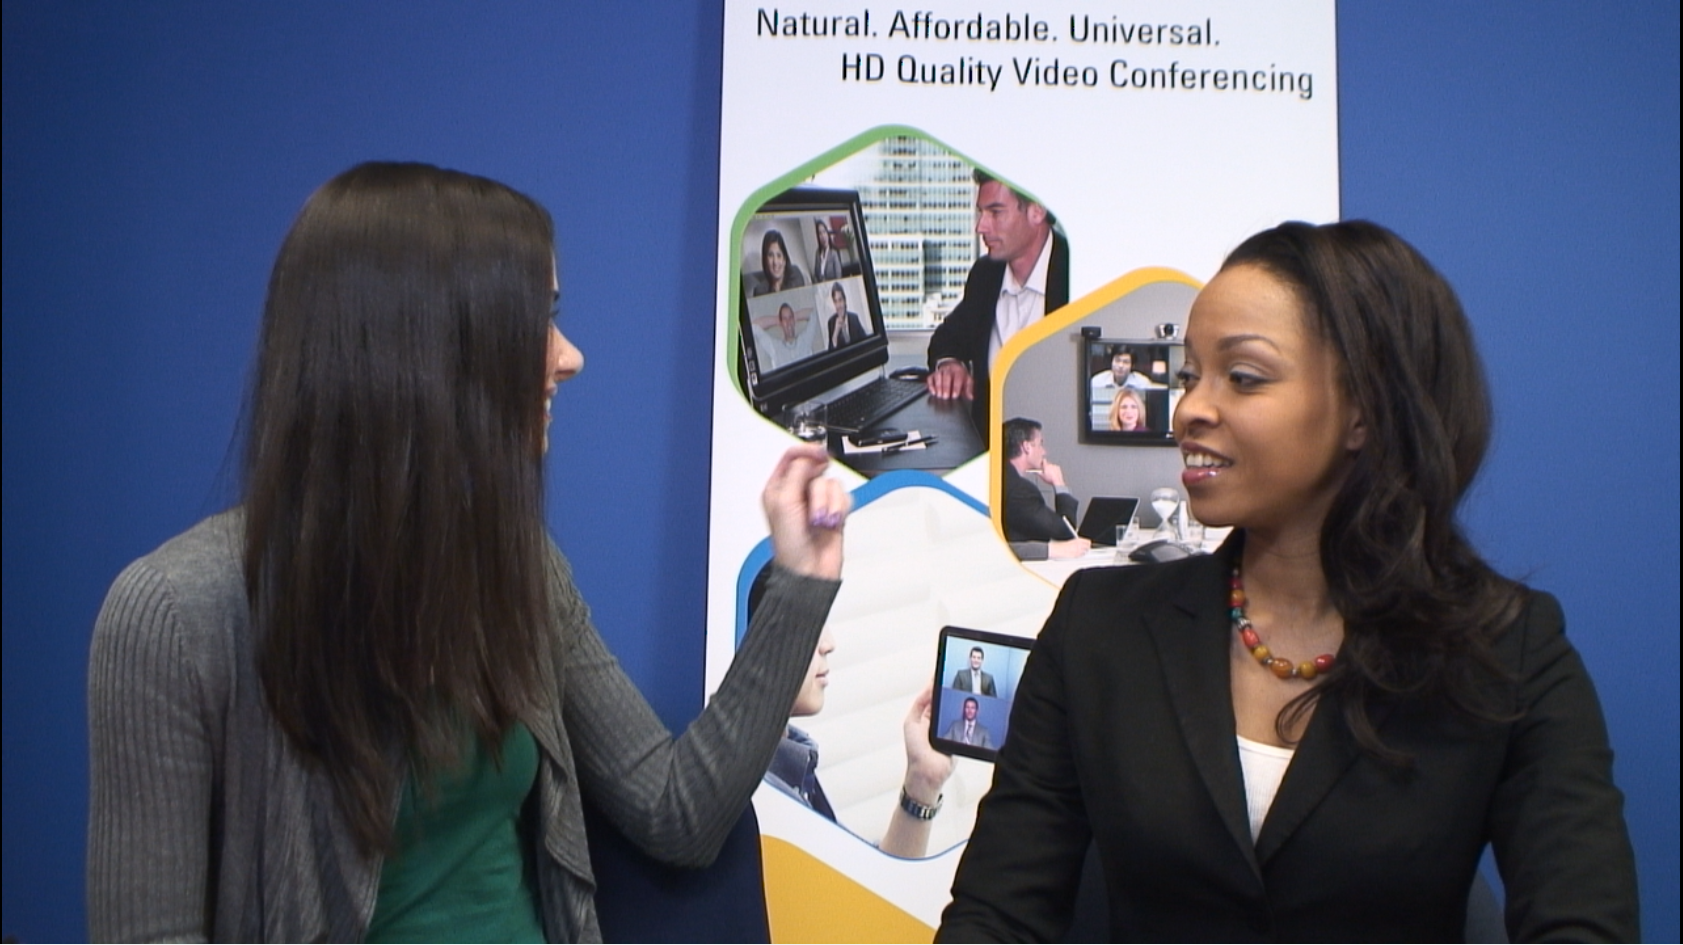
\includegraphics[width=\columnwidth]{pictures/ch6/KrsitenandSara.png}
		\label{fig:SVT-AV1_KandS}}
	\caption{Kristen and Sara from HEVC \cite{HEVCTestvideo} Video Sequence, 1280x720, 25fps}
\end{figure}





%
%                                       Chapter 7
%
\chapter{ Emerging VVC encoding standard with VMAF metric evaluation}


\begin{figure}[hbt!]
	\centering
	{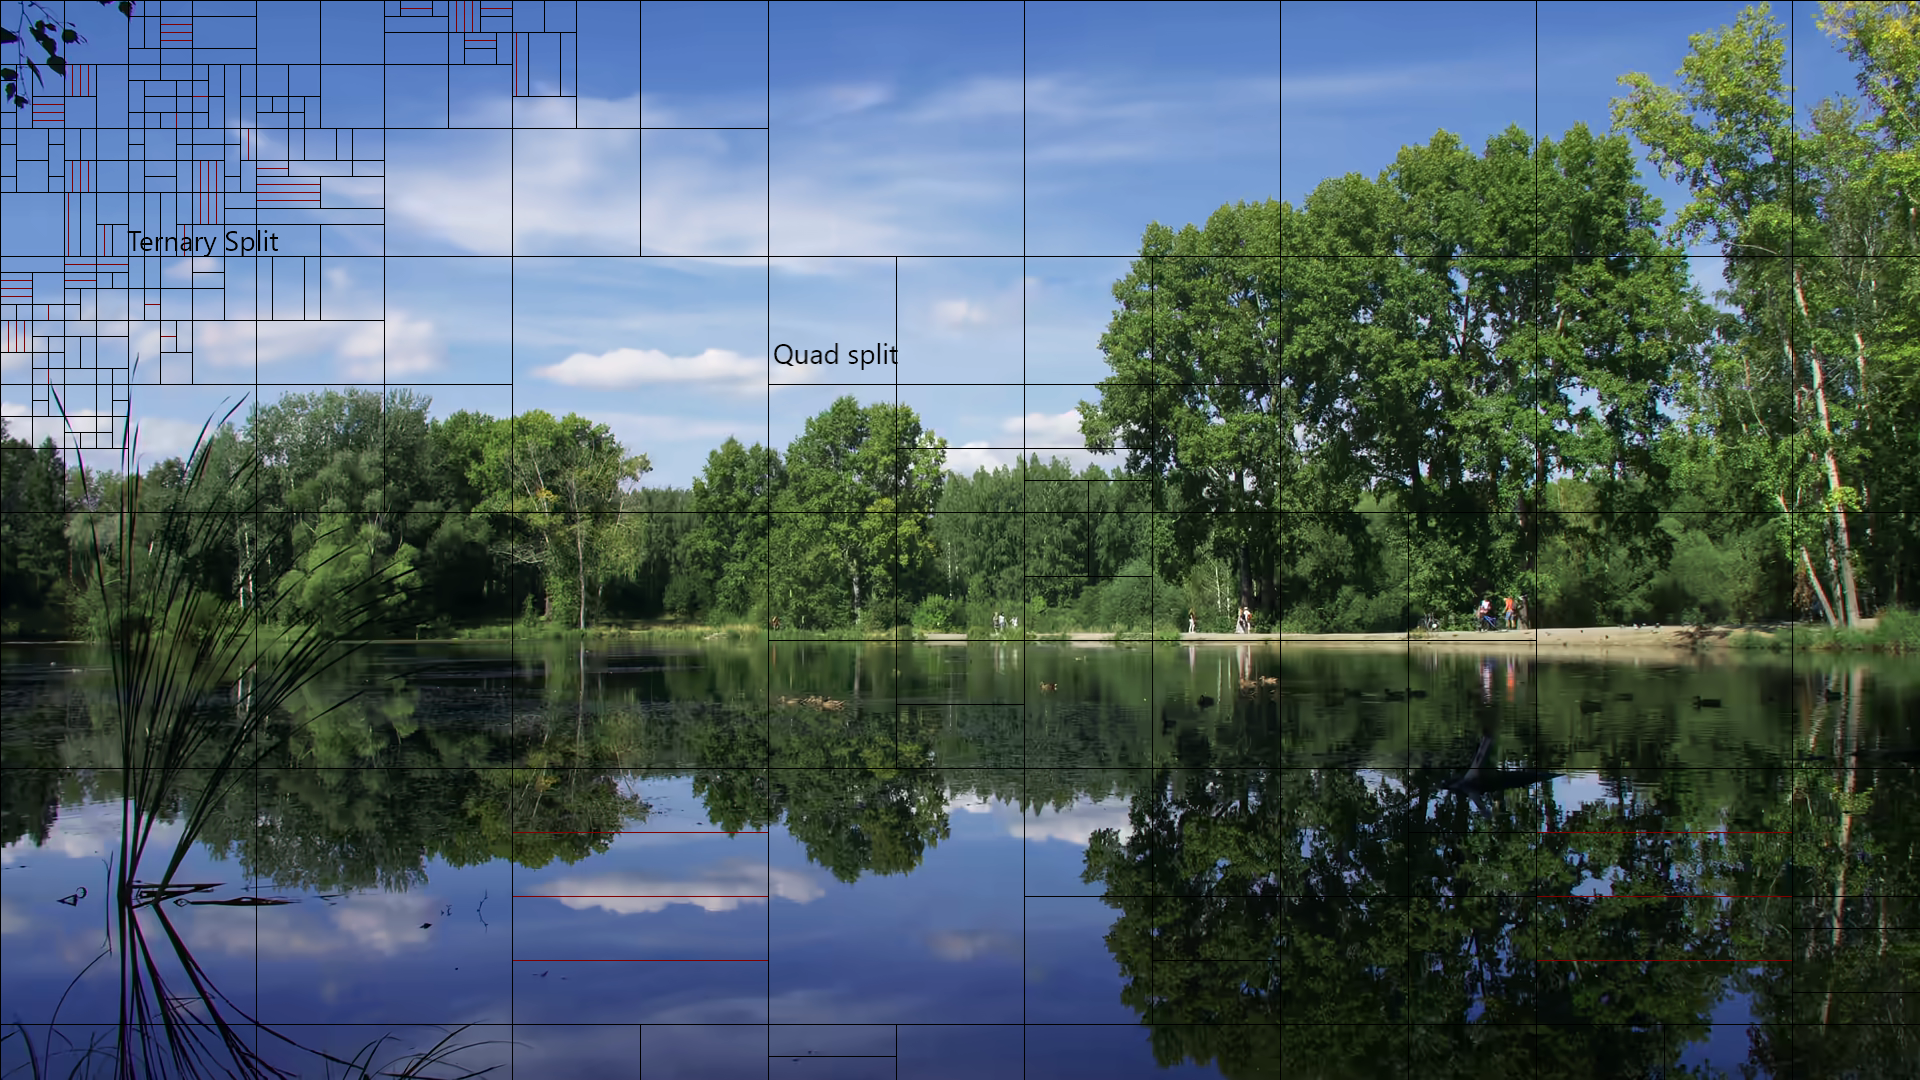
\includegraphics[width=\columnwidth]{pictures/ch7/VVC_Low_Delay_Parkrun_CTB.png}
		\label{fig:VVC_CTU}}
	\caption{CTU with Multiple Partitions-Quad and Ternary Splits in VVC.}
\end{figure}

\begin{figure}[bt!]
	\centering
	\subfloat[]
	{\includegraphics[width=1.3 true in]{pictures/ch7/ClassA_Traffic.png}
		\label{fig:Class-A1}}
	\subfloat[]
	{\includegraphics[width=1.3 true in]{pictures/ch7/ClassA_People.png}
		\label{fig:Class-A2}} 			
	\subfloat[]
	{\includegraphics[width=1.55 true in]{pictures/ch7/ClassB_Cactus.png}
		\label{fig:Class-B1}} 
	\subfloat[]
	{\includegraphics[width=1.55 true in]{pictures/ch7/ClassB_BBDrive.png}
		\label{fig:Class-B2}} \\
	\subfloat[]
	{\includegraphics[width=1.4 true in]{pictures/ch7/ClassB_Kimono.png}
		\label{fig:Class-B3}} 
	\subfloat[]
	{\includegraphics[width=1.4 true in]{pictures/ch7/ClassB_Parkrun.png}
		\label{fig:Class-B4}} 
	\subfloat[]
	{\includegraphics[width=1.4 true in]{pictures/ch7/ClassC_BQMall.png}
		\label{fig:Class-C1}}
	\subfloat[]
	{\includegraphics[width=1.4 true in]{pictures/ch7/ClassC_Party.png}
		\label{fig:Class-C2}} \\
	\subfloat[]
	{\includegraphics[width=1.4 true in]{pictures/ch7/ClassC_BBDrill.png}
		\label{fig:Class-C3}}
	\subfloat[]
	{\includegraphics[width=1.4 true in]{pictures/ch7/ClassC_Racehorse.png}
		\label{fig:Class-C4}}
	\subfloat[]
	{\includegraphics[width=1.4 true in]{pictures/ch7/ClassD_BasketballPass.png}
		\label{fig:Class-D1}}
	\subfloat[]
	{\includegraphics[width=1.4 true in]{pictures/ch7/ClassE_Johnny.png}
		\label{fig:Class-E4}}\\
	\subfloat[]
	{\includegraphics[width=1.6 true in]{pictures/ch7/ClassE_Fourppl.png}
		\label{fig:Class-E1}}
	\subfloat[]
	{\includegraphics[width=1.5 true in]{pictures/ch7/ClassE_vidyo1.png}
		\label{fig:Class-E2}}
	\subfloat[]
	{\includegraphics[width=1.5 true in]{pictures/ch7/ClassE_KandS.png}
		\label{fig:Class-E3}}
	\caption{\label{fig:HEVC_Video_Databases}
		HEVC Video Dataset with different Video resolutions and activities for BD-Rate \cite{Kalpana}
		(a),(b)Traffic, People video with resolution 2500x1600, from Class A with 25 fps,
		(c), (d), (e), (f) Cactus, Basketball Drive, Kimono, Parkrun of 1920x1080 from Class B with 50fps,
		(g) ,(h), (i), (j) BQMall, PartyScene, BasketballDrill, Racehorse of 832x480 from Class C, 		
		(k), (l),(m),(n),(o) Johnny, Four people, Vidyo1 and KristenandSara of 1280x720 from Class E with 60fps respectively. 
	}	
\end{figure}



\begin{figure}[bt!]
	\centering
	\subfloat[]
	{\includegraphics[width=1.4 true in]{pictures/ch7/Tampere_Beauty.png}
		\label{fig:Class-T1}}
	\subfloat[]
	{\includegraphics[width=1.4 true in]{pictures/ch7/Tampere_Bo.png}
		\label{fig:Class-T2}} 			
	\subfloat[]
	{\includegraphics[width=1.4 true in]{pictures/ch7/Tampere_Shake.png}
		\label{fig:Class-T3}} 
	\subfloat[]
	{\includegraphics[width=1.4 true in]{pictures/ch7/JockeyUHD.png}
		\label{fig:Class-T4}} \\
	\subfloat[]
	{\includegraphics[width=1.4 true in]{pictures/ch7/HoneyBeeUHD.png}
		\label{fig:Class-T5}} 
	\subfloat[]
	{\includegraphics[width=1.4 true in]{pictures/ch7/ReadysetGoUHD.png}
		\label{fig:Class-T6}} 
	\subfloat[]
	{\includegraphics[width=1.4 true in]{pictures/ch7/Tampere_Yacht.png}
		\label{fig:Class-T7}}	
	\caption{\label{fig:tampere_Video_Databases}
		Tampere Video, 1920x1080 Dataset  
		(a) Beauty,(b) Bo,
		(c) Shake and Dry, (d) Jockey, 
		(e) Honeybee, (f) Ready set go, (g) Yacht videos with resolution of 1920x1080 respectively \cite{UHDvideo}.}	
\end{figure}



\begin{figure}[bt!]
	\centering
	\subfloat[]
	{\includegraphics[width=1.4 true in]{pictures/ch7/UTLIVE_bs.png}
		\label{fig:Class-L1}}
	\subfloat[]
	{\includegraphics[width=1.4 true in]{pictures/ch7/UTLIVE_mc.png}
		\label{fig:Class-L2}} 			
	\subfloat[]
	{\includegraphics[width=1.4 true in]{pictures/ch7/Parkrun.png}
		\label{fig:Class-L3}} 
	\subfloat[]
	{\includegraphics[width=1.4 true in]{pictures/ch7/UTLIVE_pa.png}
		\label{fig:Class-L4}} \\
	\subfloat[]
	{\includegraphics[width=1.4 true in]{pictures/ch7/UTLIVE_rh.png}
		\label{fig:Class-L5}} 
	\subfloat[]
	{\includegraphics[width=1.4 true in]{pictures/ch7/UTLIVE_sf.png}
		\label{fig:Class-L6}} 
	\subfloat[]
	{\includegraphics[width=1.4 true in]{pictures/ch7/UTLIVE_rb.png}
		\label{fig:Class-L8}} \\
	\subfloat[]
	{\includegraphics[width=1.4 true in]{pictures/ch7/UTLIVE_st.png}
		\label{fig:Class-L9}}	
		\subfloat[]
	{\includegraphics[width=1.4 true in]{pictures/ch7/UTLIVE_sh.png}
		\label{fig:Class-L7}}
	\subfloat[]
	{\includegraphics[width=1.4 true in]{pictures/ch7/UTLIVE_tr.png}
		\label{fig:Class-L10}}	
	
	\caption{\label{fig:UTLIVE_Video_Databases}
		UT LIVE 768x432 Video Dataset  
		(a) Beauty,(b) Bo,
		(c) Shake and Dry, (d) Jockey, 
		(e) Honeybee,, (f) Ready set go, (g) Yacht videos with resolution 1920x1080 respectively.			}	
\end{figure}



\begin{figure}[hbt!]
	\centering
	\includegraphics[width=1.0\linewidth]{pictures/ch7/HEVC-240p_BD-PSNR.png}
	\caption{HEVC Dataset 240p RD Curves (PSNR vs Bitrate) of Median Values}
\label{fig:HEVC-240p-PSNR}
\end{figure}
\clearpage
\begin{figure}[hbt!]
	\centering
	\includegraphics[width=\linewidth]{pictures/ch7/HEVC-240p_BD-logPSNR.png}
	\caption{HEVC Dataset 240p RD Curves (PSNR vs Log(Bitrate) of Median Values}
	\label{fig:HEVC-240p-logPSNR}
\end{figure}

\begin{figure}[hbt!]
	\centering
	\includegraphics[width=1.0\linewidth]{pictures/ch7/HEVC-240p_BD-VMAF.png}
	\caption{HEVC Dataset 240p RD Curves (VMAF vs Bitrate) of Median Values}
\label{fig:HEVC-240p-VMAF}
\end{figure}

\begin{figure}[hbt!]
	\centering
	\includegraphics[width=1.0\linewidth]{pictures/ch7/UT_LIVE-432p_BD-PSNR1.png}
	\caption{UT LIVE RD Curves (PSNR vs Bitrate) of Median Values}
	\label{fig:UTLIVE-PSNR}
\end{figure}


\begin{figure}[hbt!]
	\centering
	\includegraphics[width=\linewidth]{pictures/ch7/UT_LIVE-432p_logPSNR.png}
	\caption{UT LIVE Dataset 432p RD Curves (PSNR vs Log(Bitrate) of Median Values}
	\label{fig:UTLIVE-432p-logPSNR}
\end{figure}


\begin{figure}[hbt!]
	\centering
	\includegraphics[width=1.0\linewidth]{pictures/ch7/UT_LIVE-432p_BD-VMAF.png}
	\caption{UT LIVE RD Curves (VMAF vs Bitrate) of Median Values}
	\label{fig:UTLIVE-VMAF}
\end{figure}

\begin{figure}[hbt!]
	\centering
	\includegraphics[width=1.0\linewidth]{pictures/ch7/HEVC-480p_BD-PSNR.png}
	\caption{HEVC Dataset 480p RD Curves (PSNR vs Bitrate) of Median Values}
\label{fig:HEVC-480p-PSNR}
\end{figure}


\begin{figure}[hbt!]
	\centering
	\includegraphics[width=\linewidth]{pictures/ch7/HEVC-480p_logPSNR.png}
	\caption{HEVC Dataset 480p RD Curves (PSNR vs Log(Bitrate) of Median Values}
	\label{fig:HEVC-480p-logPSNR}
\end{figure}


\begin{figure}[hbt!]
	\centering
	\includegraphics[width=1.0\linewidth]{pictures/ch7/HEVC-480p_BD-VMAF.png}
	\caption{HEVC Dataset 480p RD Curves (VMAF vs Bitrate) of Median Values}
\label{fig:HEVC-480p-VMAF}
\end{figure}

\begin{figure}[hbt!]
	\centering
	\includegraphics[width=1.0\linewidth]{pictures/ch7/HEVC-720p_BD-PSNR.png}
	\caption{HEVC Dataset 720p RD Curves (PSNR vs Bitrate) of Median Values}
\label{fig:HEVC-720p-PSNR}
\end{figure}


\begin{figure}[hbt!]
	\centering
	\includegraphics[width=\linewidth]{pictures/ch7/HEVC-720p_logPSNR.png}
	\caption{HEVC Dataset 720p RD Curves (PSNR vs Log(Bitrate) of Median Values}
	\label{fig:HEVC-720p-logPSNR}
\end{figure}

\begin{figure}[hbt!]
	\centering
	\includegraphics[width=1.0\linewidth]{pictures/ch7/HEVC-720p_BD-VMAF.png}
	\caption{HEVC Dataset 720p RD Curves (VMAF vs Bitrate) of Median Values}
\label{fig:HEVC-720p-VMAF}
\end{figure}


\begin{figure}[hbt!]
	\centering
	\includegraphics[width=1.0\linewidth]{pictures/ch7/HEVC-1080p_BD-PSNR.png}
	\caption{HEVC Dataset 1080p RD Curves (PSNR vs Bitrate) of Median Values}
\label{fig:HEVC-1080p-PSNR}
\end{figure}


\begin{figure}[hbt!]
	\centering
	\includegraphics[width=\linewidth]{pictures/ch7/HEVC-1080p_logPSNR.png}
	\caption{HEVC Dataset 1080p RD Curves (PSNR vs Log(Bitrate) of Median Values}
	\label{fig:HEVC-1080p-logPSNR}
\end{figure}


\begin{figure}[hbt!]
	\centering
	\includegraphics[width=1.0\linewidth]{pictures/ch7/HEVC-1080p_BD-VMAF.png}
	\caption{HEVC Dataset 1080p RD Curves (VMAF vs Bitrate) of Median Values}
\label{fig:HEVC-1080p-VMAF}
\end{figure}



\begin{figure}[hbt!]
	\centering
	\includegraphics[width=1.0\linewidth]{pictures/ch7/HEVC-1600p_BD-PSNR-Ppl.png}
	\caption{People 1600p RD Curve for (PSNR vs Bitrate) of Median Values}
\label{fig:HEVC-1600p-PSNR-Ppl}
\end{figure}

\begin{figure}[hbt!]
	\centering
	\includegraphics[width=1.0\linewidth]{pictures/ch7/HEVC-1600p_BD-logPSNR.png}
	\caption{People 1600p RD Curve for (PSNR vs Log(Bitrate) of Median Values}
	\label{fig:HEVC-1600p-logPSNR-Ppl}
\end{figure}

\begin{figure}[hbt!]
	\centering
	\includegraphics[width=1.0\linewidth]{pictures/ch7/HEVC-1600p_BD-PSNR-Traf.png}
	\caption{Traffic 1600p RD Curves (PSNR vs Bitrate) of Median Values}
	\label{fig:HEVC-1600p-PSNR-Traf}
\end{figure}

\begin{figure}[hbt!]
	\centering
	\includegraphics[width=1.0\linewidth]{pictures/ch7/HEVC-1600p_logPSNR-Traf.png}
	\caption{Traffic 1600p RD Curves (PSNR vs log Bitrate) of Median Values}
	\label{fig:HEVC-1600p-logPSNR-Traf}
\end{figure}


\begin{figure}[hbt!]
	\centering
	\includegraphics[width=1.0\linewidth]{pictures/ch7/HEVC-1600p_BD-VMAF-Ppl.png}
	\caption{People 1600p RD Curves (VMAF vs Bitrate) of Median Values}
\label{fig:HEVC-1600p-VMAF-Ppl}
\end{figure}


\begin{figure}[hbt!]
	\centering
	\includegraphics[width=1.0\linewidth]{pictures/ch7/HEVC-1600p_BD-VMAF-Traf.png}
	\caption{Traffic 1600p RD Curves (VMAF vs Bitrate) of Median Values}
	\label{fig:HEVC-1600p-VMAF}
\end{figure}

\begin{figure}[hbt!]
	\centering
	\includegraphics[width=1.0\linewidth]{pictures/ch7/BD-PSNR-BitrateGains_VVCvsAll.png}
	\caption{BD-PSNR Bitrate Gains of VVC vs All Codecs per Resolution}
	\label{fig:VVC-vs-All-PSNR}
\end{figure}

\begin{figure}[hbt!]
	\centering
	\includegraphics[width=1.0\linewidth]{pictures/ch7/BD-VMAF-BitrateGains_VVCvsAll.png}
	\caption{BD-VMAF Bitrate Gains of VVC vs All Codecs per Resolution}
	\label{fig:VVC-vs-All-VMAF}
\end{figure}


\begin{figure}[bt!]
	\centering
	\subfloat[]
	{\includegraphics[width=1.6 true in]{pictures/ch7/UTLIVE_pa.png}
		\label{fig:Shields_UTLIVE}}
	\subfloat[]
	{\includegraphics[width=1.6 true in]{pictures/ch7/Tractor_UTLIVE.png}
		\label{fig:Tractor_UTLIVE}} 			
	\subfloat[]
	{\includegraphics[width=1.6 true in]{pictures/ch7/HEVC_ClassD240.png}
		\label{fig:Bubbles}} \\
	\subfloat[]
	{\includegraphics[width=1.6 true in]{pictures/ch7/ClassA_Traffic.png}
		\label{fig:Traffic}}
	\subfloat[]
	{\includegraphics[width=1.6 true in]{pictures/ch7/ClassE_Johnny.png}
		\label{fig:Johnny}} 
	\subfloat[]
	{\includegraphics[width=1.6 true in]{pictures/ch7/ClassE_KandS.png}
		\label{fig:KS}} \\
	\subfloat[]
	{\includegraphics[width=1.6 true in]{pictures/ch7/HEVC_ClassB.png}
		\label{fig:Cac}}
	\subfloat[]
	{\includegraphics[width=1.6 true in]{pictures/ch7/ClassB_BBDrive.png}
		\label{fig:BBDrive}}
	\subfloat[]
	{\includegraphics[width=1.6 true in]{pictures/ch7/HEVC_ClassC.png}
		\label{fig:BBDrill}}\\
	\subfloat[]
	{\includegraphics[width=1.6 true in]{pictures/ch7/ClassC_Racehorse.png}
		\label{fig:RaceHorse}}
	\subfloat[]
	{\includegraphics[width=1.6 true in]{pictures/ch7/ReadysetGoUHD.png}
		\label{fig:RSG}}
		\subfloat[]
	{\includegraphics[width=1.6 true in]{pictures/ch7/HoneyBeeUHD.png}
		\label{fig:HB}}
	
	
	\caption{\label{fig:Video_Databases}
		Mixed bag video dataset for Subjective video quality assessment \cite{Kalpana}
		(a),(b)Pedestrian, Tractor, video with resolution 768x432 of 50, 25,25 fps respectively  from UT LIVE Video Quality Database .
		(c) Blowing Bubbles of 480x240 from Class D with 50fps,
		(d) Traffic of 2500x1600 from Class A with 50 fps,
		(e) ,(f) Johnny and KristenandSara of 1280x720 from Class E with 60fps, 
		(g), (h) Cactus, BasketballDrive video with resolution 1920x1080,50 fps, 
		(i), (j) Racehorse, BasketballDrill video of 832x480, 50 fps,
		(k), (l) ReadysetGo, HoneyBee videos with resolution 1920x1080 of 60 fps publicly available from Ultra Video group, Tampere University.
	}	
\end{figure}

\bibliographystyle{IEEEtran}
\bibliography{thesis1}

\end{document}
